% ACC 2027 / PaperPlaza official class. ieeeconf.cls MUST sit in the project
% root next to this file - Overleaf does not search subfolders for .cls.
\documentclass[letterpaper, 10 pt, conference]{ieeeconf}

\IEEEoverridecommandlockouts   % required before \thanks in ieeeconf
\overrideIEEEmargins           % required to meet the ACC printer margins

\usepackage{amsmath,amssymb,bm}
\let\proof\relax
\let\endproof\relax
\usepackage{amsthm} % for theorem/proof environments
\newtheorem{theorem}{Theorem}
% for theorem/proof environments
\usepackage{booktabs,array,cite}
\usepackage{graphicx}
\usepackage{float} % enables [H] (and helps with class restrictions on lone [h])
\usepackage[hidelinks]{hyperref}
% Figures live under figures/..., so keep that on the graphics path.
\graphicspath{{figures/}{figures/disturbance/}{../experiments/nengo_nef_replication_2026-08-29/results/plots/}}

% [v6] TikZ support for the architecture figures.
\usepackage{tikz}
\usepackage{verbatim}
\usetikzlibrary{arrows.meta,positioning,fit,backgrounds,calc}
% Architecture drawing helpers live in architectures/tikz/.
% Shared TikZ style for all architecture figures. Grayscale-safe.
\tikzset{
  blk/.style   ={draw,rounded corners=2pt,align=center,font=\footnotesize,
                 minimum height=8mm,inner sep=3pt,fill=white},
  clas/.style  ={blk,fill=black!4},
  neuro/.style ={blk,fill=black!12,very thick},
  plant/.style ={blk,fill=black!20},
  meas/.style  ={blk,dashed},
  sum/.style   ={draw,circle,inner sep=0pt,minimum size=4.5mm,font=\scriptsize},
  sig/.style   ={-{Latex[length=2mm]},thick},
  sigd/.style  ={-{Latex[length=2mm]},thick,dashed},
  lbl/.style   ={font=\scriptsize,inner sep=1.5pt,fill=white},
  grp/.style   ={draw,dashed,rounded corners=3pt,inner sep=6pt},
  note/.style   ={font=\scriptsize\itshape,align=left},
}


\newcommand{\R}{\mathbb R}
\newcommand{\T}{^{\mathsf T}}
\newcommand{\sat}{\operatorname{sat}}
\newcommand{\clip}{\operatorname{clip}}
\newcommand{\sgnp}{\operatorname{sgn}_{+}}

% Public code/data repository (update URL for the final version).
\newcommand{\coderepo}{\url{https://github.com/your-repo}}

\newtheorem{proposition}{Proposition}
\newtheorem{remark}{Remark}

% [v7] Title now names the mechanism and the learning, and claims the
% controlled study rather than architectural novelty.
\title{\LARGE \bf Online PES Decoder Learning in Neuromorphic Residual Control of UAV Quaternion Tracking}

% ACC/PaperPlaza template author format (ieeeconf.cls does not support IEEEtran blocks).
\author{Gandhi Contreras$^{1}$, Steven Sandoval$^{1}$, and Luis Rodolfo Garcia Carrillo$^{2}$%
\thanks{$^{1}$New Mexico State University (NMSU), Las Cruces, NM, USA.}%
\thanks{$^{2}$ Space Vehicles Directorate, Air Force Research Laboratory (AFRL), Kirtland Air Force Base (KAFB), Albuquerque, NM 87108.
    Email: {\tt\small luis\_rodolfo.garcia\_carrillo@afrl.af.mil}}%
}

\usepackage{etoolbox}
\apptocmd{\thebibliography}{\itemsep=-1pt\relax}{}{}
% [v11] Layout only: tighter float separation and fuller float pages. Template fonts unchanged.
\setlength{\textfloatsep}{6pt plus 2pt minus 2pt}
\setlength{\floatsep}{5pt plus 2pt minus 2pt}
\setlength{\intextsep}{5pt plus 2pt minus 2pt}
\setlength{\dbltextfloatsep}{6pt plus 2pt minus 2pt}
\setlength{\dblfloatsep}{5pt plus 2pt minus 2pt}
\setlength{\abovecaptionskip}{3pt}
\setlength{\belowcaptionskip}{0pt}
\renewcommand{\topfraction}{0.92}
\renewcommand{\bottomfraction}{0.5}
\renewcommand{\textfraction}{0.08}
\renewcommand{\floatpagefraction}{0.8}
\renewcommand{\dbltopfraction}{0.92}
\renewcommand{\dblfloatpagefraction}{0.8}
\begin{document}
\maketitle

% NOTE: The official ACC/PaperPlaza template often suppresses page numbers for
% submission. If you need page numbers for internal review, use `plain`.
\pagestyle{plain}
\thispagestyle{plain}

% [v7] Rewritten: leads with the mechanism and the result; scope limits kept
% but stated once rather than after every claim.
%We present a compact neuromorphic residual controller for quaternion attitude tracking with bounded actuator commands. A fixed quaternion PD baseline is augmented by six paired coupled membrane--gate (CMG) units: continuous, non-spiking, conductance-based neurons whose gate-derived activities form a nonlinear basis. Eighteen decoder weights adapt online via prescribed error sensitivity (PES), and the bounded residual is \emph{added} to the saturated baseline so the baseline is recovered exactly at zero authority. We give bounds on internal states, command deviation, and projected decoder weights, and we isolate three commonly conflated mechanisms: intrinsic conductance modulation, decoder learning, and residual authority.
%In ten matched 45-s MuJoCo cases spanning five missions on Skydio X2 and Crazyflie~2.0 models (the latter completed with an explicit four-rotor interface), CMG--PES reduces mean quaternion-angle error by $17.3$--$60.6\%$ relative to PD while respecting actuator limits (nonzero bound occupancy only in brief Hardstep intervals). Direct and Nengo implementations agree to $2.013\times10^{-6}$ relative mean error. In the tested gain regime, most of the improvement is carried by online decoder adaptation; toggling conductance modulation is numerically indistinguishable. A benchmark against LIF, ALIF, Izhikevich, and LIFRate bases shows the same hierarchy and exposes an effort--accuracy tradeoff: families that match CMG--PES on error spend several times its residual authority to do so. Noise reruns keep the reduction range at $18.1$--$55.8\%$ with seed standard deviation below $0.031\%$, and an intermittent-disturbance study shows learned corrections reused across episodes. Results are in simulation and establish boundedness, not closed-loop stability.

% Online neuromorphic residual control can augment a conventional attitude controller under abrupt missions or unforeseen disturbances without changing its feedback gains or actuator interface. We present six continuous coupled membrane-gate (CMG) units and eighteen decoder weights adapted by prescribed error sensitivity (PES), adding a bounded correction to the saturated quaternion proportional-derivative (PD) torque request before rotor-force allocation. Across ten matched 45-second MuJoCo cases on the Skydio X2 and a Crazyflie~2 derived model, mean quaternion-angle error decreases by 17.3--60.6\%, including approximately 53--57\% reductions on the Full3 and Hard45 multi-axis tracking missions. Direct and Nengo implementations agree closely. Benchmarks against LIF, ALIF, Izhikevich, and LIFRate neuron models expose an effort-accuracy tradeoff: CMG--PES attains better tracking with substantially lower realized residual effort. Under synthetic measurement noise, the error reductions persist, and learned corrections are reused across repeated disturbances. Overall, PD provides a nominal, interpretable reference, while the online residual adds bounded, revocable adaptation that improves robustness to disturbances and noisy measurements.


\begin{comment}
    The abstract of a paper should contain a description of the problem addressed, a statement of the
main result, a key conclusion that you want to highlight, and perhaps some comment on an application/
numerical example included. One or two sentences for each of these items should be sucient.
The abstract should not include literature reviews, should not attempt to justify why the problem is
important/timely, and should not discuss problems not solved in the paper.
Abstracts are often included in searchable databases and therefore should be self-contained, with
neither bibliographic citations nor references to gures/tables in the paper. Since they are often automatically
converted to pure text, equations and non-text symbols should be avoided.
The above paragraphs are not an appropriate abstract for this paper. A more suitable abstract would
be:
\The general structure of a technical paper in the control systems area is discussed. Our aim
is to assist students/researchers that are starting to write technical papers for peer reviewed
conferences or journals. We provide examples of what to include and what not to include in
each section of a technical paper."
Note that I did not start any sentence with \In this paper, . . . " This construction is generally
redundant and one can simply drop these three words. This also applies to the introduction and remaining
sections of the paper.
\end{comment}

\begin{abstract}
% 1. Description of problem addressed. 
Quadrotor attitude controllers must track time-varying references while respecting coupled rotor-force limits and coping with modeling, measurement uncertainty, and disturbances. 
% 2. Statement of the main result. 
We present an online neuromorphic residual architecture based on six continuous coupled conductance-based membrane-gate units that generate temporal features, and eighteen decoder weights adapt online through prescribed error sensitivity (PES). The decoded correction is bounded and added to a saturated PD quaternion-tracking controller before the rotor-force allocation, preserving classical feedback. A conditional local input-to-state
analysis gives explicit bounds on the attitude perturbation and residual authority under stated inertia and allocation assumptions. 
% 3. highlight conclusion and application/numerical examples
Comparisons with a tuned-PD feedforward controller show that the additional benefit of the residual is mission- and platform-dependent rather than universal.
These simulation results identify persistent temporal activity combined with online decoder learning as the principal mechanism behind the observed improvement.
\end{abstract}

\section{Introduction}

% 1. Should briefly describe the problem. The need to study the problem addressed. 
Quadrotor attitude controllers must track time-varying references while
respecting coupled rotor-force limits under modeling uncertainty, measurement
noise, and disturbances. Classical feedback provides an interpretable
stabilizing backbone, but unmodeled effects and abrupt disturbances can leave
structured tracking errors that are difficult to remove without retuning or
increasing actuator demand. Residual control offers a complementary approach:
a learned correction adapts online while preserving the classical feedback law
and actuator interface.

%Bounded authority makes the learning layer switchable; it does not by itself ensure stability or safety.

% 2. Relates the problem to the relevant literature. 
Residual learning has been combined with classical controllers in robotics
\cite{johannink2019}, including geometric $\mathcal L_1$ quadrotor
augmentation with performance guarantees \cite{wu2025l1quad} and
proportional--integral--derivative (PID) attitude control augmented by a
proximal policy optimization (PPO) residual \cite{li2027hpappo}. Neuromorphic
control provides another route for stateful adaptive corrections. Nengo
supports the Neural Engineering Framework and online decoder learning
\cite{bekolay2014nengo}, commonly using prescribed error sensitivity (PES) as
a local error-driven update \cite{voelker2015pes}. PES-based adaptive control
has been demonstrated on manipulators
\cite{dewolf2016arm,dewolf2020nengo} and in a spiking PID controller for a
free-flying UAV \cite{olivares2026selftuning}. However, continuous
membrane--gate features for actuator-aware quaternion residual control, and the
separate roles of neuron dynamics and decoder learning, remain insufficiently
characterized.


% 3. Contribution of the paper. 
%We study a bounded torque residual for quaternion attitude tracking of an unmanned aerial vehicle (UAV) with individual rotor-force saturation. The question is whether a small stateful basis improves a fixed PD controller, and whether any improvement comes from its neuron dynamics, decoder learning, or correction magnitude.
We study an online neuromorphic residual controller for quaternion attitude
tracking with individual rotor-force saturation. A quaternion
proportional--derivative (PD) controller supplies the baseline torque, six
continuous coupled membrane--gate (CMG) units generate temporal features, and
an eighteen-parameter decoder adapts online through a PES-style update. The
bounded decoder output is added to the saturated baseline before common
rotor-force allocation; setting the residual authority to zero therefore
recovers the baseline exactly. We compare the residual with both the original
fixed PD controller and a tuned PD controller with desired-rate feedforward,
separating improvement over a basic reference from additional benefit beyond a
stronger classical baseline.

The paper's contributions are:
\begin{enumerate}
    \item a fully specified CMG--PES residual architecture with paired-current
    encoding, continuous state dynamics, online decoder adaptation, bounded
    readout, and explicit rotor-force allocation, Fig. \ref{fig:arch};
    \item analytic bounds on internal states, decoder weights, and command
    deviation, including exact baseline recovery at zero residual authority;
    \item a controlled ablation separating conductance modulation, decoder
    learning, and residual authority, together with a matched neuron-family
    comparison; and
    \item a two-platform, five-mission simulation study with measurement-noise
    and repeated-disturbance experiments that evaluates the online residual as the
    classical baseline is strengthened.
\end{enumerate}

Each CMG unit couples a leaky membrane state to a gating state that modulates
its effective conductance, combining LIF-like integration with
Hodgkin--Huxley-inspired gating dynamics
\cite{hodgkin1952quantitative}. The controller uses the resulting continuous,
non-spiking trajectory as a temporal feature basis; it does not require spike
events or claim neuromorphic-hardware energy savings. In the tested regime,
online decoder adaptation is the primary source of improvement, whereas
conductance modulation has a comparatively small effect. The additional
benefit over tuned PD--feedforward control is mission- and
platform-dependent rather than universal.

The remainder of the paper is organized as follows. Section~\ref{sec:problem}
defines the attitude-tracking problem and actuator interface.
Section~\ref{sec:architecture} presents the CMG--PES architecture and learning
rule. Section~\ref{sec:analysis} establishes the boundedness properties.
Section~\ref{sec:results} reports the baseline comparisons, ablations,
neuron-family benchmark, noise experiments, and repeated-disturbance results.
Section~\ref{sec:conclusion} summarizes the findings and limitations.
Code, model files, and run archives will be available at \coderepo.


\begin{figure*}
    \centering
    % Trim bottom whitespace in the standalone PDF so the caption sits closer.
    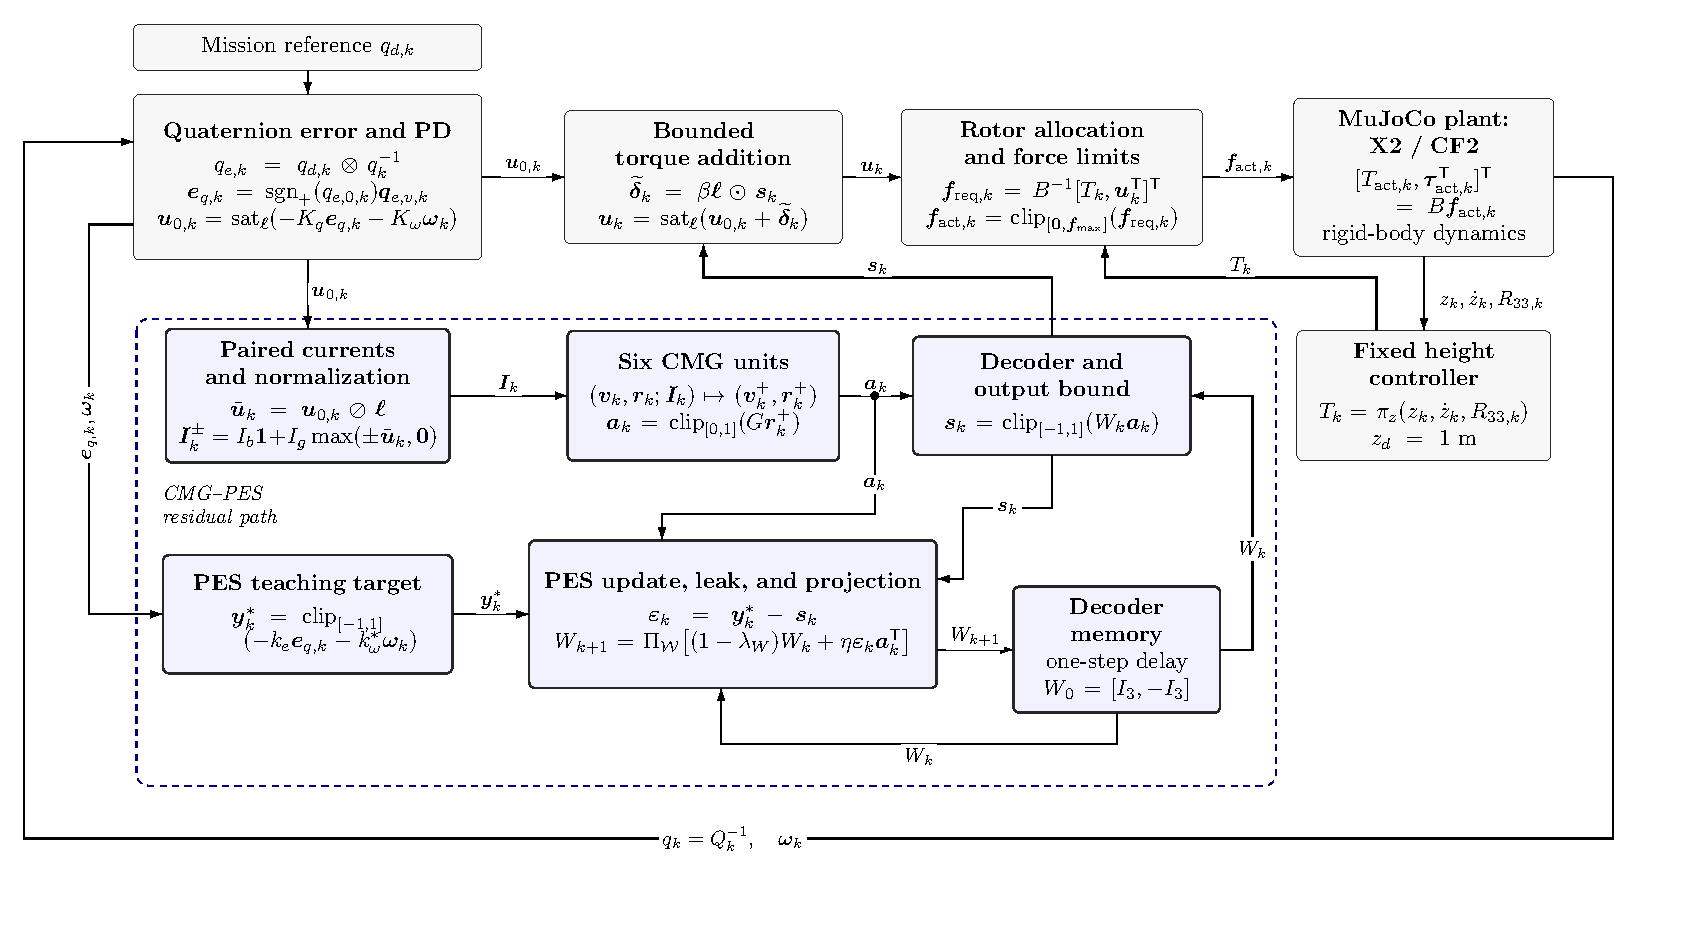
\includegraphics[width=.80\textwidth,trim=0 10mm 0 0,clip]{architectures/architecture_standalone.pdf}
    \caption{Online PES decoder learning CMG-PES Neuromorphic Residual Control architecture}
    \label{fig:arch}
\end{figure*}

\begin{comment}
\begin{figure*}[t]

\centering
\resizebox{\textwidth}{!}{% A2p -- paper variant of A2: same diagram, annotation note removed
% (it belongs in the caption). Intended for a two-column figure* at
% \textwidth; no \resizebox needed at 10pt.
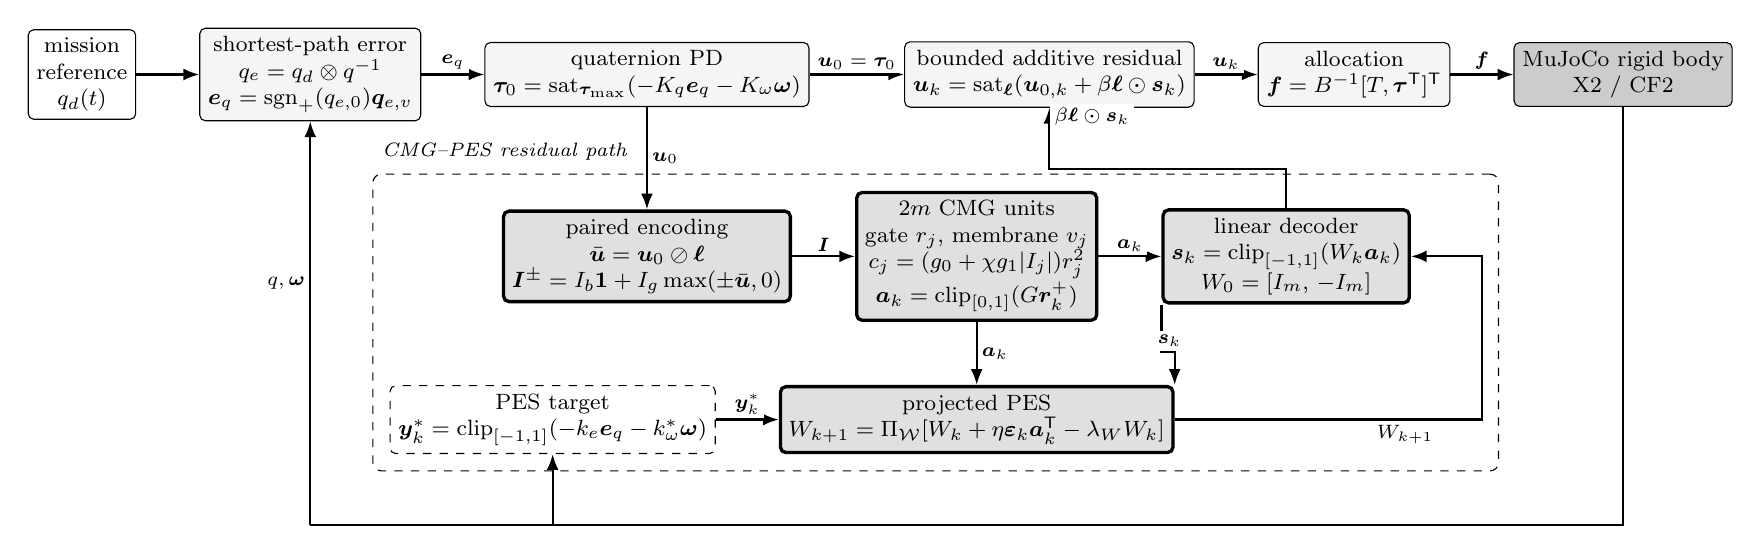
\begin{tikzpicture}[node distance=6mm and 8mm]
  \node[blk]                    (ref)  {mission\\reference\\$q_d(t)$};
  \node[clas,right=of ref]      (err)  {shortest-path error\\
                                        $q_e=q_d\otimes q^{-1}$\\
                                        $\bm e_q=\sgnp(q_{e,0})\bm q_{e,v}$};
  \node[clas,right=of err]      (pd)   {quaternion PD\\
                                        $\bm\tau_0=\sat_{\bm\tau_{\max}}(-K_q\bm e_q-K_\omega\bm\omega)$};
  \node[clas,right=12mm of pd]  (res)  {bounded additive residual\\
                                        $\bm u_k=\sat_{\bm\ell}(\bm u_{0,k}+\beta\bm\ell\odot\bm s_k)$};
  \node[clas,right=of res]      (alc)  {allocation\\$\bm f=B^{-1}[T,\bm\tau\T]\T$};
  \node[plant,right=of alc]     (plt)  {MuJoCo rigid body\\X2 / CF2};

  \node[neuro,below=13mm of pd] (enc)  {paired encoding\\
                                        $\bar{\bm u}=\bm u_0\oslash\bm\ell$\\
                                        $\bm I^{\pm}=I_b\bm 1+I_g\max(\pm\bar{\bm u},0)$};
  \node[neuro,right=of enc]     (cmg)  {$2m$ CMG units\\
                                        gate $r_j$, membrane $v_j$\\
                                        $c_j=(g_0+\chi g_1|I_j|)r_j^2$\\
                                        $\bm a_k=\clip_{[0,1]}(G\bm r_k^{+})$};
  \node[neuro,right=of cmg]     (dec)  {linear decoder\\
                                        $\bm s_k=\clip_{[-1,1]}(W_k\bm a_k)$\\
                                        $W_0=[I_m,\,-I_m]$};
  \node[neuro,below=8mm of cmg](pes)  {projected PES\\
                                        $W_{k+1}=\Pi_{\mathcal W}[W_k+\eta\bm\varepsilon_k\bm a_k\T-\lambda_W W_k]$};
  \node[meas,left=of pes]       (tgt)  {PES target\\
                                        $\bm y^*_k=\clip_{[-1,1]}(-k_e\bm e_q-k^*_\omega\bm\omega)$};

  \draw[sig] (ref) -- (err);
  \draw[sig] (err) -- node[lbl,above]{$\bm e_q$} (pd);
  \draw[sig] (pd)  -- node[lbl,above]{$\bm u_0=\bm\tau_0$} (res);
  \draw[sig] (res) -- node[lbl,above]{$\bm u_k$} (alc);
  \draw[sig] (alc) -- node[lbl,above]{$\bm f$} (plt);

  \draw[sig] (pd.south) -- node[lbl,right]{$\bm u_0$} (enc.north);
  \draw[sig] (enc) -- node[lbl,above]{$\bm I$} (cmg);
  \draw[sig] (cmg) -- node[lbl,above]{$\bm a_k$} (dec);
  \draw[sig] (dec.north) -- ++(0,5mm) -| node[lbl,pos=.93,right]{$\beta\bm\ell\odot\bm s_k$} (res.south);
  \draw[sig] (cmg.south) -- node[lbl,right]{$\bm a_k$} (pes.north);
  \draw[sig] (tgt) -- node[lbl,above]{$\bm y^*_k$} (pes);
  \draw[sig] (dec.south west) -- ++(0,-6mm) -| node[lbl,pos=.3,above]{$\bm s_k$} (pes.north east);
  \coordinate (wx) at ($(dec.east)+(9mm,0)$);
  \draw[sig] (pes.east) -- node[lbl,pos=.75,below]{$W_{k+1}$} (pes.east-|wx) -- (wx) -- (dec.east);

  \coordinate (busy) at ($(pes.south)+(0,-9mm)$);
  \draw[thick] (plt.south) -- (plt|-busy) -- (err|-busy);
  \draw[sig]   (err|-busy) -- node[lbl,pos=.6,left]{$q,\bm\omega$} (err.south);
  \draw[sig]   (tgt|-busy) -- (tgt.south);

  \begin{scope}[on background layer]
    \node[grp,fit=(enc)(cmg)(dec)(pes)(tgt)(wx)] (nb) {};
  \end{scope}
  \node[note,anchor=south west] at ([yshift=0.5mm]nb.north west)
    {CMG--PES residual path};
\end{tikzpicture}
}
\caption{CMG--PES residual architecture. The light blocks are the fixed
classical path: error \eqref{eq:theta}, PD law \eqref{eq:pd}, and
allocation \eqref{eq:mixer} are never adapted. The heavy blocks encode the
clipped baseline as paired currents \eqref{eq:encoding}, evolve $2m$
membrane--gate units \eqref{eq:cmg}, and decode a bounded residual
\eqref{eq:readout} that is \emph{added} to the saturated baseline
\eqref{eq:residual}. Only $W_k$ adapts, through \eqref{eq:pes}; $\beta=0$
recovers the baseline exactly.}
\label{fig:arch}
\end{figure*}
\end{comment}

% [v6] fig:scale and fig:models were merged: both showed the same two
% aircraft. The old fig:scale call sites now point here.
\begin{figure*}[t]
\centering
% Fig. 2 (standalone PDF in figures/01_mujoco_missions/)
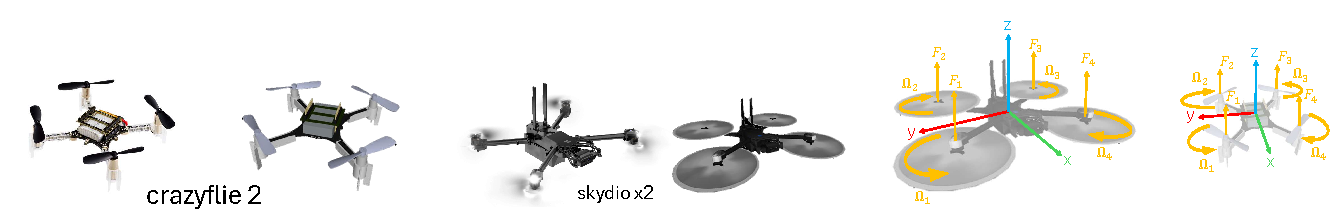
\includegraphics[width=.60\textwidth]{figures/01_mujoco_missions/fig2_drones_only.pdf}

\caption{Vehicles and simulation models. Left: CF2 hardware and MuJoCo
model. Centre: X2 hardware and MuJoCo model. Right: both geometries at
relative scale. The axis triads are body-frame axes: they are rigidly
attached to the vehicle and therefore rotate with it relative to the
inertial (world) frame (cf.\ $Q\!:\,\text{body}\to\text{inertial}$ in
Sec.~\ref{sec:problem}).}
\label{fig:models}
\end{figure*}


%%%%%%%%%%%%%%%%%%%%%%%%%%%%%%%%%%%%%%%%%%%%%%%%%%%%%%%%%%%%%%%%%%%%%%%%%%
% [v6] Nomenclature. Every symbol that appears in an equation is listed
% once here; the bracketed tag is the equation that defines it.

\begin{comment}
\begin{table*}[t]
\caption{Nomenclature. Parenthesised tags give the defining equation;
vectors are bold; $\clip_{[a,b]}$ and $\sat_{\bm\ell}$ act elementwise.}
\label{tab:nomen}\centering\scriptsize
\setlength{\tabcolsep}{4pt}
\renewcommand{\arraystretch}{0.84}
\begin{tabular}{@{}l>{\raggedright\arraybackslash}p{0.185\textwidth}l>{\raggedright\arraybackslash}p{0.185\textwidth}l>{\raggedright\arraybackslash}p{0.185\textwidth}@{}}
\toprule
\multicolumn{6}{@{}l}{\textit{Attitude, plant, and notation}}\\
$q,\;q_d$ & state / reference quaternion & $q_e$ & error quaternion, $q_d\otimes q^{-1}$ & $q_{e,0},\bm q_{e,v}$ & scalar and vector parts\\
$\bm e_q$ & shortest-path error \eqref{eq:theta} & $\theta_q$ & error angle \eqref{eq:theta} & $\bm\omega$ & body angular rate\\
$J$ & inertia tensor & $Q$ & body-to-inertial rotation & $\otimes$ & quaternion product\\
$\bm\omega_d,\bm\omega_e$ & reference and error rate \eqref{eq:errkin} & $R(\cdot)$ & rotation matrix of a quaternion & $z,z_d,\dot z$ & height, reference, rate \eqref{eq:collective}\\
$\odot,\oslash$ & elementwise $\times$, $\div$ & $\sgnp$ & sign, with $\sgnp(0)=1$ & $\sigma$ & logistic function\\
$I_m$ & identity of order $m$ & $\R$ & real numbers & $\Pi$ & Euclidean projection\\
\midrule
\multicolumn{6}{@{}l}{\textit{Fixed baseline and actuator interface}}\\
$\bm\tau_0=\bm u_0$ & baseline torque \eqref{eq:pd} & $K_q,K_\omega$ & PD gains \eqref{eq:pd} & $\bm\tau_{\max}$ & per-axis torque bound\\
$\omega_n,\zeta$ & design frequency, damping & $\bm\ell$ & per-channel command bound & $\sat_{\bm\ell}$ & saturation at $\pm\bm\ell$\\
$B$ & allocation matrix \eqref{eq:allocationmatrix} & $\bm f$ & rotor forces \eqref{eq:mixer} & $T$ & collective thrust \eqref{eq:collective}\\
$\kappa_i$ & rotor reaction coefficient & $m$ & torque channels, $m=3$ & $M$ & vehicle mass\\
$\bm f_{\max}$ & per-rotor force bound & $g$ & gravity, $9.81$\,m/s$^2$ & $\bm 1$ & vector of ones\\
\midrule
\multicolumn{6}{@{}l}{\textit{Coupled membrane--gate unit}}\\
$v_j$ & membrane state \eqref{eq:cmg} & $r_j$ & gate state \eqref{eq:cmg} & $c_j$ & shunt conductance \eqref{eq:cmg}\\
$\bar{\bm u}$ & normalized baseline \eqref{eq:encoding} & $\bm I^{\pm},\bm I$ & paired currents \eqref{eq:encoding} & $I_b,I_g$ & current offset and gain\\
$\tau,\tau_r$ & membrane, gate time constants & $v_{\rm th}$ & gate threshold & $v_{\rm rest},v_{\rm reset}$ & rest level, reversal level\\
$\gamma$ & gate self-coupling & $\alpha_h$ & logistic sharpness & $\chi$ & conductance switch, $\chi\in\{0,1\}$\\
$g_0,g_1$ & conductance gains (distinct from $g$) & $G$ & activity gain, $G=10^5$ & $h$ & integration step\\
$b_{j,k}$ & gate target \eqref{eq:gate_step} & $r^+_{j,k},v^+_{j,k}$ & updated states \eqref{eq:mem_step} & $\lambda_{j,k},d_{j,k}$ & frozen membrane coefficients\\
\midrule
\multicolumn{6}{@{}l}{\textit{Decoder, online learning, and residual authority}}\\
$\bm a_k$ & clipped activity \eqref{eq:readout} & $W_k$ & decoder \eqref{eq:readout} & $W_0$ & initial decoder, $[I_m,-I_m]$\\
$\bm s_k$ & clipped readout \eqref{eq:readout} & $\bm y^*_k$ & PES target \eqref{eq:pes} & $\bm\varepsilon_k$ & PES error \eqref{eq:pes}\\
$k_e,k^*_\omega$ & target gains \eqref{eq:pes} & $\eta$ & per-step learning rate & $\lambda_W$ & per-step decoder decay\\
$\Pi_{\mathcal W},W_{\max}$ & projection and weight bound & $\beta$ & residual authority \eqref{eq:residual} & $\bm u_k,\bm\delta_k$ & applied command, deviation \eqref{eq:residual}\\
\midrule
\multicolumn{6}{@{}l}{\textit{Reported metrics}}\\
$\bar\theta_q$ & mean quaternion-angle error & $S$ & actuator-bound occupancy [\%] & $n$ & runs per reported cell\\
\bottomrule
\end{tabular}
\end{table*}
\end{comment}


%%%%%%%%%%%%%%%%%%%%%%%%%%%%%%%%%%%%%%%%%%%%%%%%%%
\section{Attitude Baseline and Actuator Interface}
\label{sec:problem}
%%%%%%%%%%%%%%%%%%%%%%%%%%%%%%%%%%%%%%%%%%%%%%%%%%

The objective is to reduce shortest-path attitude error for a prescribed
$q_d(t)$ while respecting rotor-force limits. Baseline and augmented
controllers share the state measurements, height loop, and allocator;
Section~\ref{sec:architecture} modifies only the requested attitude torque.

%\input{figure1_interface.tex}

\subsection{Quaternion Convention and Error}

Let $Q\in\mathbb S^3$ be the scalar-first Hamilton quaternion mapping body to
inertial coordinates, and let $\bm\omega$ be the body angular velocity. The
rotational dynamics are \cite{schaub2018amss}
\begin{align}
 \dot Q&=\tfrac12 Q\otimes[0,\bm\omega\T]\T,\\
 \bm J\dot{\bm\omega}&=\bm\tau_{\rm act}+\bm\tau_{\rm p}
       +\bm\tau_{\rm d}-\bm\omega\times(\bm J\bm\omega).
 \label{eq:plant}
\end{align}
where $\bm J\succ0$ is the body-frame inertia, $\bm u$ is the commanded
body torque, and $\bm\tau_{\rm act}$ is the torque realized after rotor
allocation and force clipping; hence $\bm\tau_{\rm act}=\bm u$ when the
request is feasible and generally $\bm\tau_{\rm act}\neq\bm u$ otherwise.
The terms $\bm\tau_{\rm p}$ and $\bm\tau_{\rm d}$ denote modeled passive and
externally applied disturbance torques, respectively.

Using the corresponding passive quaternion $q=Q^{-1}$, define
%\cite{diebel2006quaternion}
\begin{equation}
 \dot q=-\tfrac12[0,\bm\omega\T]\T\otimes q.
 \label{eq:passive}
\end{equation}
The desired attitude $q_d$ uses the same convention. Define the attitude error
\begin{align}
 q_e&=q_d\otimes q^{-1}=[q_{e,0},\bm q_{e,v}\T]\T,\\
 \bm e_q&=\sgnp(q_{e,0})\bm q_{e,v},\qquad \sgnp(0)=1,\\
 \theta_q&=2\operatorname{atan2}(\|\bm q_{e,v}\|_2,|q_{e,0}|)
             \in[0,\pi].
 \label{eq:theta}
\end{align}
The metric $\theta_q$ is invariant to the quaternion sign. The sign selection
is nonsmooth at $q_{e,0}=0$; the analysis below is therefore local and does
not establish global hybrid stability \cite{mayhew2011hybrid}.
%The reported error $\theta_q$ is the shortest rotation angle, invariant under $q_e\mapsto-q_e$. Sign selection introduces a discontinuity at $q_{e,0}=0$; it does not establish robust hybrid global stability \cite{mayhew2011hybrid}.

For a desired-frame rate $\bm\omega_d$ satisfying the corresponding passive kinematics, differentiation gives
\begin{align}
 \dot q_e&=\tfrac12q_e\otimes[0,\bm\omega_e\T]\T,\\
 \bm\omega_e&=\bm\omega-R(q_e)\T\bm\omega_d,\qquad
 \dot q_{e,0}=-\tfrac12\bm q_{e,v}\T\bm\omega_e.
 \label{eq:errkin}
\end{align}
These are kinematic identities (no convergence implied). Reference Euler triples parameterize $q_d$ in this passive convention.

\subsection{Physical Inertia and Implemented PD Gains}
Let $\bm J\succ0$ denote the rigid-body inertia about the center of mass, expressed in body axes \cite{schaub2018amss}. When principal moments $\bm j_{\rm p}$ are specified in a rotated principal-axis frame, the physical body-frame tensor is
\begin{equation}
 \bm J=R_{BI}\operatorname{diag}(\bm j_{\rm p})R_{BI}\T,
 \label{eq:inertiaframe}
\end{equation}
for the rotation from principal axes to body axes $R_{BI}$. The implementation sets axiswise gains using the principal moments in their reported ordering, $\bm j_{\rm tune}$, not necessarily $\operatorname{diag}(\bm J)$ (Table~\ref{tab:models}).

The fixed quaternion PD baseline is
\begin{align}
 \bm k_q&=2\bm j_{\rm tune}\odot\bm\omega_n^2,\qquad
 \bm k_\omega=2\zeta\bm j_{\rm tune}\odot\bm\omega_n,\\
 \bm u_0&=\sat_{\bm\ell}
       (-\bm k_q\odot\bm e_q-\bm k_\omega\odot\bm\omega),
 \label{eq:pd}
\end{align}
where $\odot$ denotes componentwise multiplication,
$\bm\omega_n=(4,4,3.5)\T$ rad/s, $\zeta=0.95$, and
$\sat_{\bm\ell}$ clips component $i$ to $[-\ell_i,\ell_i]$.
%
The requested-torque box is $\mathcal U=\prod_{i=1}^3[-\ell_i,\ell_i]$;
$\clip_{[a,b]}$ also acts componentwise, and $\oslash$ denotes componentwise division.
We impose componentwise torque limits $\bm\ell\in\mathbb R_{>0}^3$ through $\sat_{\bm\ell}(\cdot)$. In our implementation, $\bm\ell$ is chosen proportional to the diagonal gain-scheduling vector $\bm j_{\rm tune}$ via
$\ell_i=\max(j_{{\rm tune},i}\nu_i,10^{-6}\ \mathrm{N\,m})$,
with acceleration-scale vector $\bm\nu=(12,12,10)\T$ rad/s$^2$.
These controller-side bounds are not the rotor-feasible torque set.
%
The law is quaternion feedback \cite{fresk2013quaternion}; $\bm\omega_n$ is a tuning parameter rather than a claimed set of coupled closed-loop natural frequencies.
Equation~\eqref{eq:pd} damps the absolute body rate, whereas \eqref{eq:errkin} defines the rate error $\bm\omega_e$. A residual that corrects a baseline missing that term would be credited with work the baseline could do itself, so the study also carries the feedforward law
\begin{equation}
 \bm u_0^{\rm ff}=\sat_{\bm\ell}\bigl(-\bm k_q\odot\bm e_q-\bm k_\omega\odot(\bm\omega-\bm\omega_d)\bigr),
 \label{eq:pdff}
\end{equation}
with $\bm\omega_d$ obtained by central differences of the reference, and a bandwidth-scaled variant $\bm\omega_n\!\mapsto\!\rho\bm\omega_n$. Gyroscopic cancellation remains omitted.
The resulting gains are vehicle-specific through $\bm j_{\rm tune}$, even though
$\bm\omega_n$ and $\zeta$ are shared; the same fixed gains are then retained
for PD and its CMG augmentation.
The local result in Section~\ref{sec:local} uses these anisotropic gains; it does not replace them with a scalar-gain controller.
%
\subsection{Requested and Realized Wrench}
For rotor positions $\bm p_i$ in body coordinates, parallel $+z$ thrust
axes, and signed reaction coefficients $\kappa_i$, define
\begin{equation}
 B=\begin{bmatrix}
 1&1&1&1\\p_{1,y}&p_{2,y}&p_{3,y}&p_{4,y}\\
 -p_{1,x}&-p_{2,x}&-p_{3,x}&-p_{4,x}\\
 \kappa_1&\kappa_2&\kappa_3&\kappa_4
 \end{bmatrix}.
 \label{eq:allocationmatrix}
\end{equation}
The signs follow $\bm p_i\times[0,0,f_i]\T$ and the actuator's local reaction torque $\kappa_i f_i$. Here $B$ maps rotor thrusts to total thrust and body torque; $\kappa_i$ has units of meters, not angular velocity. Given a commanded collective thrust $T$ and body-torque command $\bm u$, the corresponding inverse-allocation and clipping model is
\begin{equation}
 \begin{aligned}
 \bm f_{\rm req}&=B^{-1}[T,\bm u\T]\T,\\
 \bm f_{\rm act}&=\clip_{[\bm0,\bm f_{\max}]}(\bm f_{\rm req}),\\
 [T_{\rm act},\bm\tau_{\rm act}\T]\T&=B\bm f_{\rm act}.
 \end{aligned}
 \label{eq:mixer}
\end{equation}
Here $\bm u=\bm u_0$ for PD; the CMG path in Section~\ref{sec:architecture}
modifies that requested torque before the same allocation and clipping.
Each $f_i$ is a commanded force in newtons, not a rotor-speed command.
Exact wrench realization requires
$B^{-1}[T,\bm u\T]\T\in[\bm0,\bm f_{\max}]$.
A componentwise torque box is not generally contained in this
collective-dependent feasible set. Clipped inverse allocation is used,
not an optimization-based allocator \cite{monteiro2016allocation}.

Collective thrust remains classical, with $z_d=1$ m:
\begin{equation}
 T=\clip_{[0,2.5Mg]}
 \left(\frac{M[g+6(z_d-z)-4\dot z]}{\max(R(Q)_{33},0.35)}\right).
 \label{eq:collective}
\end{equation}
Here $g$ is the gravitational acceleration. The height loop reads altitude and vertical velocity; the denominator compensates tilt.
The guard $0.35$ prevents near-singular tilt compensation as $R(Q)_{33}\to0$
(i.e., near $90^\circ$ tilt) and corresponds to limiting the effective
compensation to about $\arccos(0.35)\approx69.5^\circ$. Its upper bound does
not supersede individual rotor limits. The CMG path has no direct collective
output, but can affect height through attitude, tilt compensation, and
allocation saturation.
The resulting shared plant interface isolates changes in requested
attitude torque while preserving the same physical simulation for both
controllers.

%%%%%%%%%%%%%%%%%%%%%%%%%%%%%%%%%%%%%%%%%%%%%%%%%%%%%%%%%%%%%%%%%
\section{CMG State Dynamics and Online Decoder Adaptation}
\label{sec:architecture}
\label{sec:analysis}
%%%%%%%%%%%%%%%%%%%%%%%%%%%%%%%%%%%%%%%%%%%%%%%%%%%%%%%%%%%%%%%%%
This section specifies the residual architecture in state-space form and the online decoder update, then states the boundedness properties that follow from the resulting saturations and projections.
\subsection{Encoding, States, and Numerical Update}

For $m$ torque channels and $2m$ units, normalize the clipped baseline and
form positive/negative current pairs:
\begin{equation}
 \begin{aligned}
 \bar{\bm u}&=\bm u_0\oslash\bm\ell,\\
 \bm I^{\pm}&=I_b\bm1+I_g\max(\pm\bar{\bm u},\bm0),\\
 \bm I&=[(\bm I^+)\T,(\bm I^-)\T]\T.
 \end{aligned}
 \label{eq:encoding}
\end{equation}
Each unit has a dimensionless membrane state $v_j$ and gate $r_j$:
\begin{align}
 \dot r_j&=[\sigma(\alpha_h(v_j-v_{\rm th}+\gamma r_j))-r_j]/\tau_r,\\
 \dot v_j&=-(v_j-v_{\rm rest})/\tau+I_j/\tau-c_j(v_j-v_{\rm reset}),\\
 c_j&=(g_0+\chi g_1|I_j|)r_j^2,\qquad \chi\in\{0,1\}.
 \label{eq:cmg}
\end{align}
% [v6] CMG unit coupling topology (TikZ source under architectures/tikz/).
\begin{figure}[t]
\centering
\resizebox{0.86\columnwidth}{!}{% B1c -- column-native CMG unit: coupling topology only. The state
% equations stay in the text; the figure shows which variable acts on which.
% Natural width is about one IEEE column, so no \resizebox is needed.
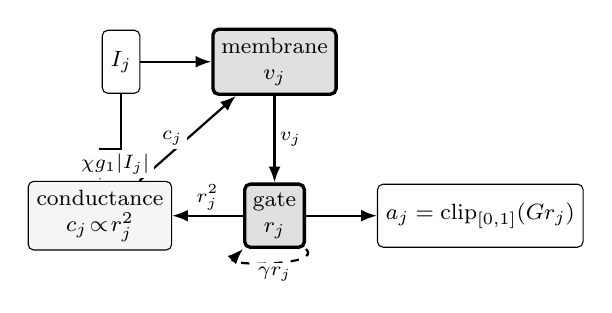
\begin{tikzpicture}[node distance=6mm and 9mm,font=\footnotesize]
  \node[blk]                       (I) {$I_j$};
  \node[neuro,right=of I]          (v) {membrane\\$v_j$};
  \node[neuro,below=11mm of v]     (r) {gate\\$r_j$};
  \node[clas,left=of r]            (c) {conductance\\$c_j\!\propto\! r_j^{2}$};
  \node[blk,right=of r]            (a) {$a_j=\clip_{[0,1]}(G r_j)$};

  \draw[sig] (I) -- (v);
  \draw[sig] (v.south) -- node[lbl,right]{$v_j$} (r.north);
  \draw[sig] (r) -- node[lbl,above]{$r_j^{2}$} (c);
  \draw[sig] (c) -- node[lbl,left]{$c_j$} (v);
  \draw[sig] (r) -- (a);
  \draw[sigd] (r.south east) to[out=-45,in=-135]
        node[lbl,below]{$\gamma r_j$} (r.south west);
  \draw[sig] (I.south) -- ++(0,-7mm) -| node[lbl,pos=.14,below]{$\chi g_1|I_j|$} (c.north);
\end{tikzpicture}
}
\caption{Coupling topology of one CMG unit, cf.~\eqref{eq:cmg}. The
membrane sets the gate target; the gate acts back twice, shifting its own
threshold through $\gamma$ and shunting the membrane through
$c_j\propto r_j^2$ ($\chi=1$ makes that shunt input dependent). The
dynamics are continuous: no spike, no reset, and only $a_j$ leaves the
unit.}
\label{fig:cmgunit}
\end{figure}
%
The logistic gate target depends on $v_j$, while $r_j$ shifts that target
and modulates membrane conductance (Fig.~\ref{fig:cmgunit}). Thus, both states participate even
though the decoder reads the gate-derived activity. The model has no
threshold-triggered reset or spike event; $v_{\rm reset}$ is a reversal
level in a continuous conductance term. The gains $g_0,g_1$ have the units
needed to make $c_j$ a rate.

The actual integration is sequential, not exponential Euler for both
states. From the old states compute
\begin{align}
 b_{j,k}&=\sigma\!\left(\clip_{[-60,60]}
       [\alpha_h(v_{j,k}-v_{\rm th}+\gamma r_{j,k})]\right),\\
 r_{j,k}^{+}&=\clip_{[0,1]}
       [r_{j,k}+(h/\tau_r)(b_{j,k}-r_{j,k})].
 \label{eq:gate_step}
\end{align}
Then evaluate $c_{j,k}=(g_0+\chi g_1|I_{j,k}|)(r_{j,k}^{+})^2$,
$\lambda_{j,k}=\tau^{-1}+c_{j,k}$, and
$d_{j,k}=(v_{\rm rest}+I_{j,k})/\tau+c_{j,k}v_{\rm reset}$. The
frozen-coefficient membrane step is
\begin{equation}
 v_{j,k}^{+}=e^{-\lambda_{j,k}h}v_{j,k}
       +(1-e^{-\lambda_{j,k}h})d_{j,k}/\lambda_{j,k}.
 \label{eq:mem_step}
\end{equation}
This exactly solves the scalar membrane equation with those frozen
coefficients; it does not establish unconditional stability of the coupled
nonlinear closed loop. Assign $(v_{j,k+1},r_{j,k+1})=(v_{j,k}^{+},r_{j,k}^{+})$.

\subsection{Readout, PES, and Additive Residual}
The within-step activity, initial decoder, and clipped readout are
\begin{equation}
 \begin{aligned}
 \bm a_k&=\clip_{[0,1]}(G\bm r_k^+),\qquad W_0=[I_m,-I_m],\\
 \bm s_k&=\clip_{[-1,1]}(W_k\bm a_k).
 \end{aligned}
 \label{eq:readout}
\end{equation}
Pair subtraction retains directional information from a nonnegative
activity basis; state memory does not imply instantaneous sign agreement
after a command reversal. With $G=10^5$ the activity saturates once
$r_j\ge10^{-5}$, so $G$ is a primary design hyperparameter for how much of
$r_j$'s dynamic range reaches the decoder. The teaching target and local update are
\begin{align}
 \bm y_k^*&=\clip_{[-1,1]}(-k_e\bm e_{q,k}-k_\omega^*\bm\omega_k),\\
 \bm\varepsilon_k&=\bm y_k^*-\bm s_k,\\
 W_{k+1}&=\Pi_{\mathcal W}
       [W_k+\eta\bm\varepsilon_k\bm a_k\T-\lambda_W W_k].
 \label{eq:pes}
\end{align}
Here $\mathcal W=[-W_{\max},W_{\max}]^{m\times2m}$. The coefficients $\eta$ and $\lambda_W$ are per-step (so changing $h$ changes the effective learning dynamics). PES is a local error-driven update toward the prescribed target $\bm y_k^*$; it does not differentiate through the plant or claim to minimize a closed-loop cost.

Using $W_k$ before the update, the requested command is
\begin{equation}
 \bm u_k=\sat_{\bm\ell}(\bm u_{0,k}+\beta\bm\ell\odot\bm s_k),\quad
 \bm\delta_k=\bm u_k-\bm u_{0,k},\quad 0\le\beta\le1.
 \label{eq:residual}
\end{equation}
The canonical UAV case has $m=3$, six CMG units, and eighteen decoder
weights. Intrinsic conductance modulation ($\chi$), synaptic/decoder
adaptation ($W_k$), and output authority ($\beta\bm\ell$) are distinct.

\subsection{Structural Properties and Their Scope}
We first state the boundedness properties that follow directly from the architecture: internal-state bounds, a uniform command-deviation bound set by residual authority, and projection-based bounds on decoder weights.
\begin{proposition}[Bounded internal states]\label{prop:states}
With the nonnegative conductance parameters in Table~\ref{tab:parameters},
$r_{j,0}\in[0,1]$, and $0<h\le\tau_r$, the gate remains in $[0,1]$.
The membrane iterate remains in the convex hull of its initial value,
$v_{\rm reset}$, and the interval
$[v_{\rm rest}+I_b,v_{\rm rest}+I_b+I_g]$.
\end{proposition}
\begin{proof}
The unclipped gate step is a convex combination of $r_{j,k}$ and
$b_{j,k}\in[0,1]$. Since $I_j\in[I_b,I_b+I_g]$ and $c_j\ge0$,
$d_j/\lambda_j$ is a convex combination of $v_{\rm rest}+I_j$ and
$v_{\rm reset}$. Equation~\eqref{eq:mem_step} is a convex combination of
$v_{j,k}$ and $d_j/\lambda_j$. Induction proves both statements.
\end{proof}

\begin{proposition}[Bounded authority and baseline recovery]
\label{prop:authority}
For $\bm u_{0,k}\in\mathcal U$ and any finite $W_k$,
$\bm u_k\in\mathcal U$ and $|\delta_{k,i}|\le\beta\ell_i$.
If $\beta=0$, the requested baseline command is recovered at every step.
If $W_k=0$ at a particular step, it is recovered at that step, but learning
need not keep $W_{k+1}=0$.
\end{proposition}
\begin{proof}
The outer clip enforces membership in $\mathcal U$. Its componentwise
nonexpansiveness and $\sat_{\ell_i}(u_{0,k,i})=u_{0,k,i}$ give
$|\delta_{k,i}|\le|\beta\ell_i s_{k,i}|\le\beta\ell_i$.
The recovery statements follow by substitution.
\end{proof}
The same allocator and state then give the same actuator output when
$\beta=0$. The proposition does not establish state safety, rotor
headroom, stability, or a bound on tracking improvement. A bounded
adversarial correction can still degrade or destabilize a nonlinear plant.

\begin{proposition}[Decoder bound and restricted contraction]
\label{prop:pes}
If $W_0\in\mathcal W$, then \eqref{eq:pes} keeps $W_k\in\mathcal W$.
If, additionally, the target and a nonzero activity $\bm a$ are fixed,
leak is zero, and readout clipping and projection remain inactive, then
\begin{equation}
 \bm\varepsilon_{k+1}
       =(1-\eta\|\bm a\|_2^2)\bm\varepsilon_k.
 \label{eq:contraction}
\end{equation}
For a nonzero initial error, its norm contracts to zero when
$0<\eta\|\bm a\|_2^2<2$.
\end{proposition}
\begin{proof}
Projection gives the first result. Under the additional conditions,
$(W_{k+1}-W_k)\bm a=\eta\bm\varepsilon_k\|\bm a\|_2^2$;
subtracting this from the fixed target error gives
\eqref{eq:contraction}. The scalar multiplier has modulus less than one
under the stated condition.
\end{proof}
This is the constant-feature PES result \cite{voelker2015pes}, not a
closed-loop convergence theorem. Since $\|\bm a\|^2\le2m$,
$0<\eta<1/m$ is sufficient for that restricted model with nonzero
activity; changing targets, loss of excitation, clipping, and leakage
invalidate a direct application to the experiment. No unique identification
of all decoder weights follows from one fixed regressor.

% [v7] The statement a control audience looks for first. Scoped: it is a
% conditional bound, not a stability theorem, and says so.
%\begin{remark}[Scope of a small-gain argument]
%\label{rem:smallgain}
%Propositions~\ref{prop:authority} and \ref{prop:pes} place the realized
%command deviation in a known box, $|\delta_{k,i}|\le\beta\ell_i$, uniformly
%in $k$ and independently of what the decoder has learned. If the baseline
%loop is input-to-state stable with respect to an additive torque
%perturbation, with gain $\gamma(\cdot)$ on that input, then the augmented
%loop inherits an ISS estimate with asymptotic bound
%$\gamma(\beta\|\bm\ell\|)$, and $\beta$ tunes it continuously to zero. Two
%conditions are not discharged here. The perturbation entering the plant is
%post-allocation, so the relevant bound is on $B^{-1}$ applied to
%$\bm\delta_k$ under rotor saturation, not on $\bm\delta_k$ itself; and the
%required ISS gain for the saturated quaternion-PD baseline is not
%established in this paper. The architecture therefore supplies the bounded
%perturbation such an argument needs, and identifies the two missing
%ingredients, without asserting the conclusion.
%\end{remark}

\subsection{Allocation-Aware Local Stability}
\label{sec:local}
Let $E=[\bm0_{3\times1},I_3]\T$, $H=E\T$, and let
$\mathcal A_T(\bm u)=HB\clip_{[0,\bm f_{\max}]}(B^{-1}[T,\bm u\T]\T)$
be the realized torque at collective $T$. For two commands at the
\emph{same state and collective}, scalar clipping has secant slopes
$d_i\in[0,1]$. Consequently,
\begin{align}
 \mathcal A_T(\bm u)-\mathcal A_T(\bm u_0)
 &=HBDB^{-1}E\bm\delta,\\
 \|\mathcal A_T(\bm u)-\mathcal A_T(\bm u_0)\|_2
 &\le L_A\beta\|\bm\ell\|_2,
 \label{eq:allocbound}
\end{align}
where $D=\operatorname{diag}(d_i)$ and
$L_A=\max_{D\in\mathcal D}\|HBDB^{-1}E\|_2$.
$\mathcal D$ is the set of sixteen diagonal matrices with entries
in $\{0,1\}$. The vertex maximum bounds all intermediate $D$ by convexity.
This holds even with rotor clipping, but is not a bound between two
different closed-loop trajectories. It also does not bound the height error.

For a constant reference and a smooth shortest-path branch, let
$\bm x=[\bm e_q\T,\bm\omega\T]\T$ and
$K_q=\operatorname{diag}(\bm k_q)$, $K_\omega=\operatorname{diag}(\bm k_\omega)$.
Write the continuous-time attitude subsystem as
\begin{equation}
 \begin{gathered}
 \dot{\bm x}=A\bm x+\bm g(\bm x)+F\bm d,\\
 A=\begin{bmatrix}0&\frac12I_3\\-\bm J^{-1}K_q&-\bm J^{-1}K_\omega\end{bmatrix},
 \qquad F=\begin{bmatrix}0\\\bm J^{-1}\end{bmatrix},
 \end{gathered}
 \label{eq:localmodel}
\end{equation}
where $\bm d=\bm\tau_{\rm act}+\bm\tau_{\rm p}+\bm\tau_{\rm d}
 +K_q\bm e_q+K_\omega\bm\omega$ is the total deviation from ideal PD torque.
It includes allocation and command-saturation errors, not just the neural
request. The nonlinear remainder is
\begin{equation}
 \bm g(\bm x)=\begin{bmatrix}
 \tfrac12[(\sqrt{1-\|\bm e_q\|^2}-1)I_3+[\bm e_q]_\times]\bm\omega\\
 -\bm J^{-1}[\bm\omega]_\times\bm J\bm\omega
 \end{bmatrix}=O(\|\bm x\|^2),
 \label{eq:localremainder}
\end{equation}
with $[\bm z]_\times\bm y=\bm z\times\bm y$. Norms below use fixed
coordinates with angular rates expressed in rad/s.

\begin{theorem}[Conditional local practical stability]
\label{thm:local}
Let $\bm J,K_q,K_\omega\succ0$, let $q_d$ be constant, and use the smooth
branch in \eqref{eq:localmodel}. Choose $Q_L\succ0$ and the solution
$P\succ0$ of $A\T P+PA=-Q_L$. On $\|\bm x\|\le r<1$, suppose
$\|\bm g(\bm x)\|\le L_r\|\bm x\|^2$ and choose $r$ so that
$c=\lambda_{\min}(Q_L)-2\|P\|L_r r>0$.
Set $p_- =\lambda_{\min}(P)$, $p_+=\lambda_{\max}(P)$,
$b=\|PF\|$, and $V=\bm x\T P\bm x$. If
\begin{equation}
 V(0)\le p_-r^2,\qquad
 \|\bm d(t)\|\le\bar d<\frac{cr}{2b}\sqrt{\frac{p_-}{p_+}},
 \label{eq:localsmallness}
\end{equation}
then $V\le p_-r^2$ is forward invariant and
\begin{equation}
 V(t)\le e^{-\alpha t}V(0)+\frac{4p_+b^2}{c^2}\bar d^2,
 \qquad \alpha=\frac{c}{2p_+}.
 \label{eq:localiss}
\end{equation}
Thus attitude regulation is locally input-to-state stable; zero
perturbation gives local exponential convergence of the plant state.
\end{theorem}
\begin{proof}
The linear system has energy
$\frac12\bm\omega\T\bm J\bm\omega+\bm e_q\T K_q\bm e_q$ with derivative
$-\bm\omega\T K_\omega\bm\omega$. Its only invariant zero-derivative
trajectory is the origin, so $A$ is Hurwitz and $P\succ0$ exists.
Equations~\eqref{eq:localmodel}--\eqref{eq:localremainder} give
\[
 \dot V\le-c\|\bm x\|^2+2b\|\bm x\|\bar d
 \le-\frac c2\|\bm x\|^2+\frac{2b^2}{c}\bar d^2.
\]
On $V=p_-r^2$, $\|\bm x\|\ge r\sqrt{p_-/p_+}$, so
\eqref{eq:localsmallness} makes the first bound strictly negative.
The ellipsoid stays inside the radius-$r$ ball; integration of
$\dot V\le-\alpha V+2b^2\bar d^2/c$ gives \eqref{eq:localiss}.
\end{proof}

If the same-state baseline deviation from ideal PD is bounded by $\bar d_0$,
then \eqref{eq:allocbound} permits
$\bar d=\bar d_0+L_A\beta\|\bm\ell\|$ in the theorem, \emph{provided}
\eqref{eq:localsmallness} holds. This is a sufficient local robustness
condition, independent of the particular PES trajectory, not a PES
convergence proof. Numerical checks confirm that $A$ is Hurwitz for both
implemented gain sets. The smallness condition has not been certified
for the experimental $\beta=0.5$. Moving references, the $180^\circ$
sign boundary, sampled-data/solver error, and full translational stability
remain outside this result; sample-and-hold error would need its own
bound within $\bm d$.

\paragraph{Nengo realization.}
In Nengo~4.1.0, a custom \texttt{NeuronType} exposes membrane and gate states. Direct current injection into \texttt{ensemble.neurons} bypasses NEF gain/intercept fitting. Unfiltered CMG activity uses $\eta_N=\eta(2m)/h$ and Nengo error $\bm s-\bm y^*$. Leak uses pre-step weights; projection follows the simulator step. Nengo's teaching graph introduces a one-step latency, so this is not an identical weight sequence. The maximum relative mean-error difference over ten direct/Nengo cases is $2.013\times10^{-6}$, a tested numerical agreement rather than formal backend equivalence.


\section{Experimental Protocol and Cross-Mission Results}
\label{sec:results}
\subsection{Models, Parameters, and Measurements}

MuJoCo provides rigid-body simulation with site-applied actuator wrenches \cite{todorov2012mujoco}. We evaluate two Menagerie-derived multirotor models \cite{menagerieModels} (CF2 and X2) as free-flying rigid bodies: the attitude loop commands three body torques and a separate height loop commands collective thrust.

The upstream CF2 model exposes abstract moment channels \cite{menagerieCF2}; we replace them with four rotor-force channels and the shared clipped inverse allocator \eqref{eq:mixer} to expose thrust/torque coupling and per-rotor limits. Rotor ordering is $(-x,-y),(-x,+y),(+x,+y),(+x,-y)$ with reaction signs $(-,+,-,+)$. Table~\ref{tab:models} separates simulation/interface parameters from manufacturer context; the CF2 $1.5\times$ scale increases a model limit, not measured hardware capability. Both models are simplified (no motor/RPM/battery states and no validated rotor aerodynamics); feedback uses \texttt{qpos}/\texttt{qvel}, with noise injected only in Sec.~\ref{sec:noise}.

\begin{table}[t]
\centering
\caption{Model/interface parameters with manufacturer context (top) and the canonical 3-channel CMG--PES parameters (bottom). Neural states and currents are normalized model variables; learning coefficients are per step.
Mass agrees with published CF2/X2 specifications \cite{bitcrazeCF20Specs,skydioX2ESpecs}; force limits, inertias, and reaction coefficients are simulation parameters, not identified hardware ratings.}
\label{tab:models}\label{tab:parameters}
\setlength{\tabcolsep}{3pt}
\footnotesize
\begin{tabular}{@{}p{0.40\linewidth}p{0.27\linewidth}p{0.25\linewidth}@{}}
\toprule
Parameter & CF2 rotor model & X2 model\\
\midrule
Mass $M$ (kg) & $0.027$ & $1.325$\\
Rotor $|p_x|,|p_y|$ (m) & $0.0325,0.0325$ & $0.14,0.18$\\
Reaction magnitude $|\kappa_i|$ (m) & $0.005$ & $0.0201$\\
Rotor force limit (N) & $.0875\to.13125$ & $13$\\
Total force limit (N) & $.350\to.525$ & $52$\\
Main-test thrust/weight & $1.982$ & $4.001$\\
$\bm j_{\rm tune}$ ($10^{-5}$ kg\,m$^2$) & $(2.3951,\allowbreak2.3951,\allowbreak3.2347)$ & ---\\
$\bm j_{\rm tune}$ ($10^{-2}$ kg\,m$^2$) & --- & $(6.0711,\allowbreak3.6468,\allowbreak2.5412)$\\
Rigid-body integrator & RK4 & Euler\\
Experiment timestep (s) & $0.0005$ & $0.0005$\\
Manufacturer thrust data & $.568$ N\textsuperscript{a} & Not published\textsuperscript{b}\\
\bottomrule
\end{tabular}
\par\smallskip
\begin{minipage}{0.97\linewidth}
\scriptsize
\textsuperscript{a}Historical CF2 measurement at 93.75\% PWM using an external power supply \cite{bitcrazeThrustMeasurements}; not a continuous battery-powered rating. The modeled $.525$ N is below that observation.
\textsuperscript{b}Not reported in the reviewed X2 datasheet. Neither model includes motor lag; a historical CF2 motor step took about 180 ms \cite{bitcrazeMotorResponse}, illustrating an omitted hardware effect.
\end{minipage}
\par\medskip
\footnotesize\setlength{\tabcolsep}{3pt}
\begin{tabular}{@{}ll@{\hspace{6pt}}ll@{}}
\toprule
CMG--PES & Value & & Value\\\midrule
$h$, duration & $0.0005$ s, $45$ s & $\alpha_h,\gamma,g_0,g_1$ & $50,2,120,30$\\
$\tau,\tau_r$ & $0.05$ s, $0.005$ s & $I_b,I_g,G$ & $0.75,1.25,10^5$\\
$v_{\rm rest},v_{\rm reset},v_{\rm th}$ & $0,0,1$ & $\beta,\eta$ & $0.5,8\times10^{-4}$\\
$v_{j,0},r_{j,0},\chi$ & $0,0,1$ & $\lambda_W,W_{\max},k_e,k^*_\omega$ & $10^{-6},6,8,0$\\
\bottomrule
\end{tabular}
\end{table}

\begin{comment}
\begin{table}[t]
\centering
\caption{Simulation-model characteristics. CF2 authority is scaled relative to the upstream model limit.}
\label{tab:models}
\setlength{\tabcolsep}{3pt}
\footnotesize
\begin{tabular}{@{}p{0.40\linewidth}p{0.27\linewidth}p{0.25\linewidth}@{}}
\toprule
Property & CF2 rotor model & X2 model\\
\midrule
Mass $M$ (kg) & $0.027$ & $1.325$\\
Rotor $|p_x|,|p_y|$ (m) & $0.0325,0.0325$ & $0.14,0.18$\\
Reaction magnitude $|\kappa_i|$ (m) & $0.005$ & $0.0201$\\
Unscaled rotor limit (N) & $0.0875$ & $13$\\
Main-test authority scale & $1.5$ & $1$\\
Main-test rotor limit (N) & $0.13125$ & $13$\\
Main-test total limit (N) & $0.525$ & $52$\\
Maximum thrust/weight & $1.321\to1.982$ & $4.001$\\
Rigid-body integrator & RK4 & Euler\\
Experiment timestep (s) & $0.0005$ & $0.0005$\\
Motor activation/RPM states & None & None\\
\bottomrule
\end{tabular}
\end{table}

\begin{table}[t]
\centering
\caption{Simulation parameters vs. manufacturer information (where available).}
\label{tab:manufacturer}
\setlength{\tabcolsep}{3pt}
\footnotesize
\begin{tabular}{@{}>{\raggedright\arraybackslash}p{0.25\linewidth}>{\raggedright\arraybackslash}p{0.30\linewidth}>{\raggedright\arraybackslash}p{0.37\linewidth}@{}}
\toprule
Quantity & Simulation & Manufacturer information\\
\midrule
CF2 mass & $27$ g & $27$ g \cite{bitcrazeCF20Specs}\\
X2 mass & $1325$ g & $1325$ g with battery \cite{skydioX2ESpecs}\\
CF2 total thrust & $0.350\to0.525$ N & $0.568$ N measured at $93.75\%$ PWM\textsuperscript{a} \cite{bitcrazeThrustMeasurements}\\
X2 rotor limit & $13$ N per rotor & Not reported \cite{skydioX2ESpecs}\\
CF2 motor response & No motor dynamics & $\sim180$ ms: $0\to25{,}000$ RPM\textsuperscript{b} \cite{bitcrazeMotorResponse}\\
Inertia tensors & CF2 inherited; X2 geometry-derived & Not reported in product specifications \cite{bitcrazeCF20Specs,skydioX2ESpecs}\\
\bottomrule
\end{tabular}
\par\smallskip
\begin{minipage}{0.97\linewidth}
\scriptsize
\textsuperscript{a}Historical total-thrust measurement with a power-supply test setup, not a guaranteed continuous battery-powered rating.
\textsuperscript{b}One motor's reported full-command response with a charged battery; not an identified first-order time constant.
\end{minipage}
\end{table}
\end{comment}

CF2's body axes are principal axes. For X2, the geometry-derived body tensor is
\[
 \bm J=10^{-2}\begin{bmatrix}3.66517&0&-.21000\\0&2.54117&0\\-.21000&0&6.05280\end{bmatrix}
 \ \mathrm{kg\,m^2}.
\]
It differs from both $\operatorname{diag}(\bm j_{\rm tune})$ and a
manufacturer-identified tensor. Torque limits use $\bm j_{\rm tune}$ as
defined in Section~\ref{sec:problem}.

Each PD/CMG pair uses the same initial state, reference, duration, allocator, model, and timestep. The primary campaign is nominal and deterministic (no injected disturbances or sensor noise), with one run per cell and learning active throughout. We report the mean error $\bar\theta_q$ and relative reduction $100(\bar\theta_{q,\rm PD}-\bar\theta_{q,\rm CMG})/\bar\theta_{q,\rm PD}$; means use all 90{,}000 samples even when plotted traces are decimated.



The five reference triples are generated as follows (radians):
Roll is $(0.25\sin0.7t,0,0)$; Full3 is
$0.5\sin(t+(0,\pi/2,\pi)\T)$, componentwise. Hard45 is
\begin{equation}
 \begin{bmatrix}
 0.55\sin(0.75t)+0.20\sin(2.10t+0.40)\\
 0.45\sin(0.95t+\pi/3)+0.18\sin(1.75t)\\
 0.65\sin(0.55t+\pi)+0.25\sin(1.35t+0.20)
 \end{bmatrix}.
\end{equation}
Hardstep holds zero for one second, then cycles every two seconds through
the rows of
\begin{equation}
 \begin{bmatrix}
 .75&-.45&.55\\-.65&.55&-.70\\.50&.50&.90\\-.80&-.35&.20
 \end{bmatrix}.
\end{equation}
Yaw360 is $(0,0,2\pi(3\xi^2-2\xi^3))$ with $\xi=t/45$.
The nominal Hover equilibrium is also available, but its essentially zero
error does not support a meaningful percentage comparison.

\begin{figure}[t]
\centering
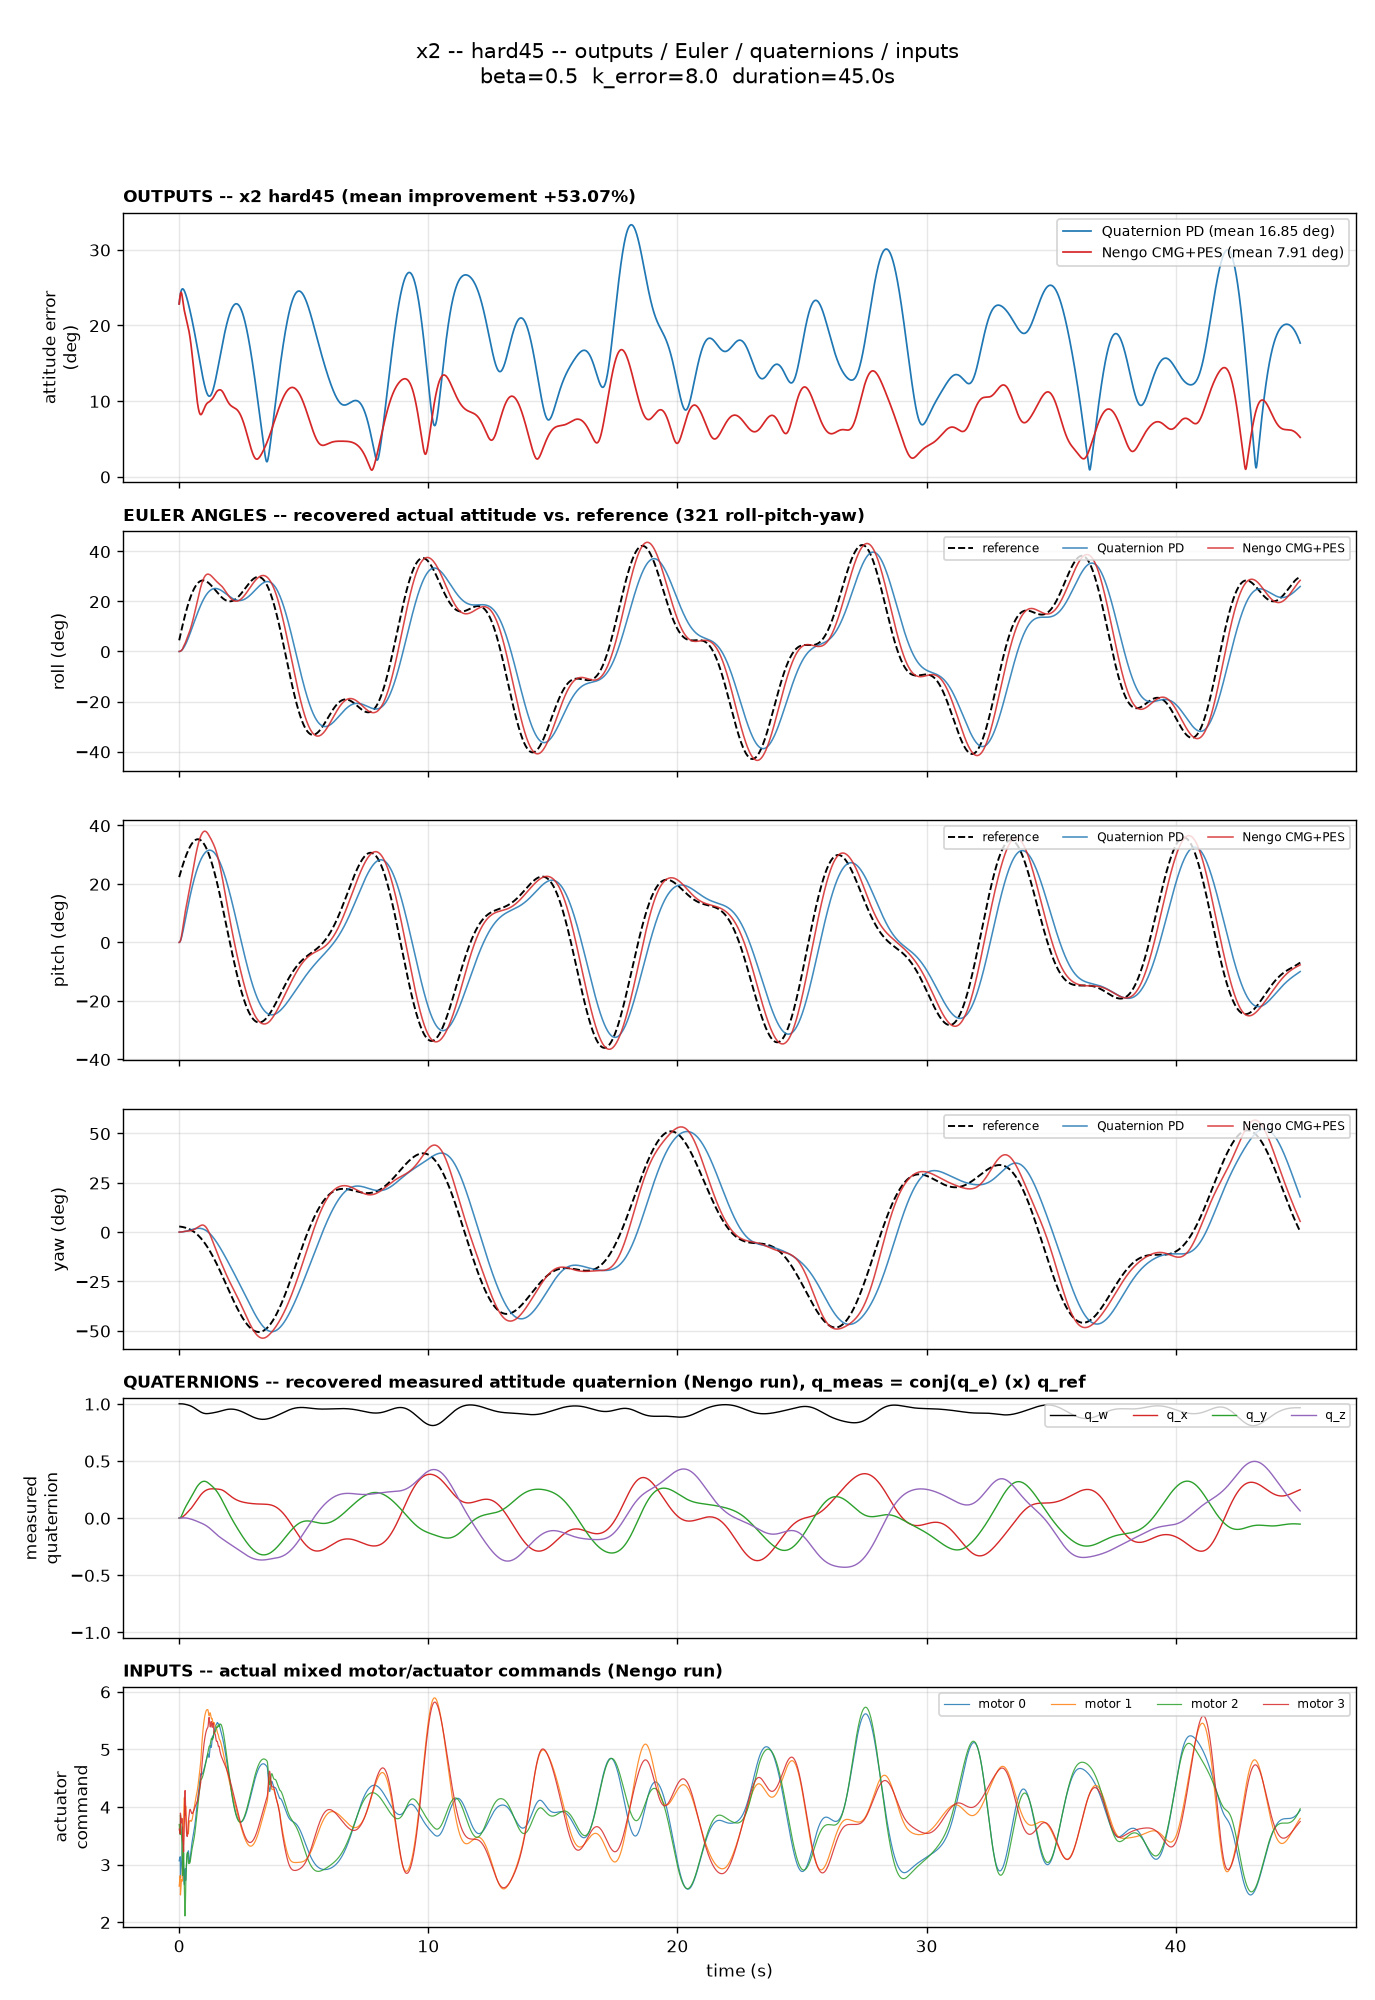
\includegraphics[width=.92\linewidth]{figures/02_neural_activity/attitude_detail/x2_hard45_attitude.png}
\caption{X2 Hard45 mission: PD baseline versus CMG--PES augmentation over the
45-s run. Hard45 commands all three axes simultaneously and delivers a large
mean-error reduction that is also relatively insensitive to measurement noise
(see Table~\ref{tab:all}).}
\label{fig:tracking}
\end{figure}

\begin{figure*}[t]
\centering
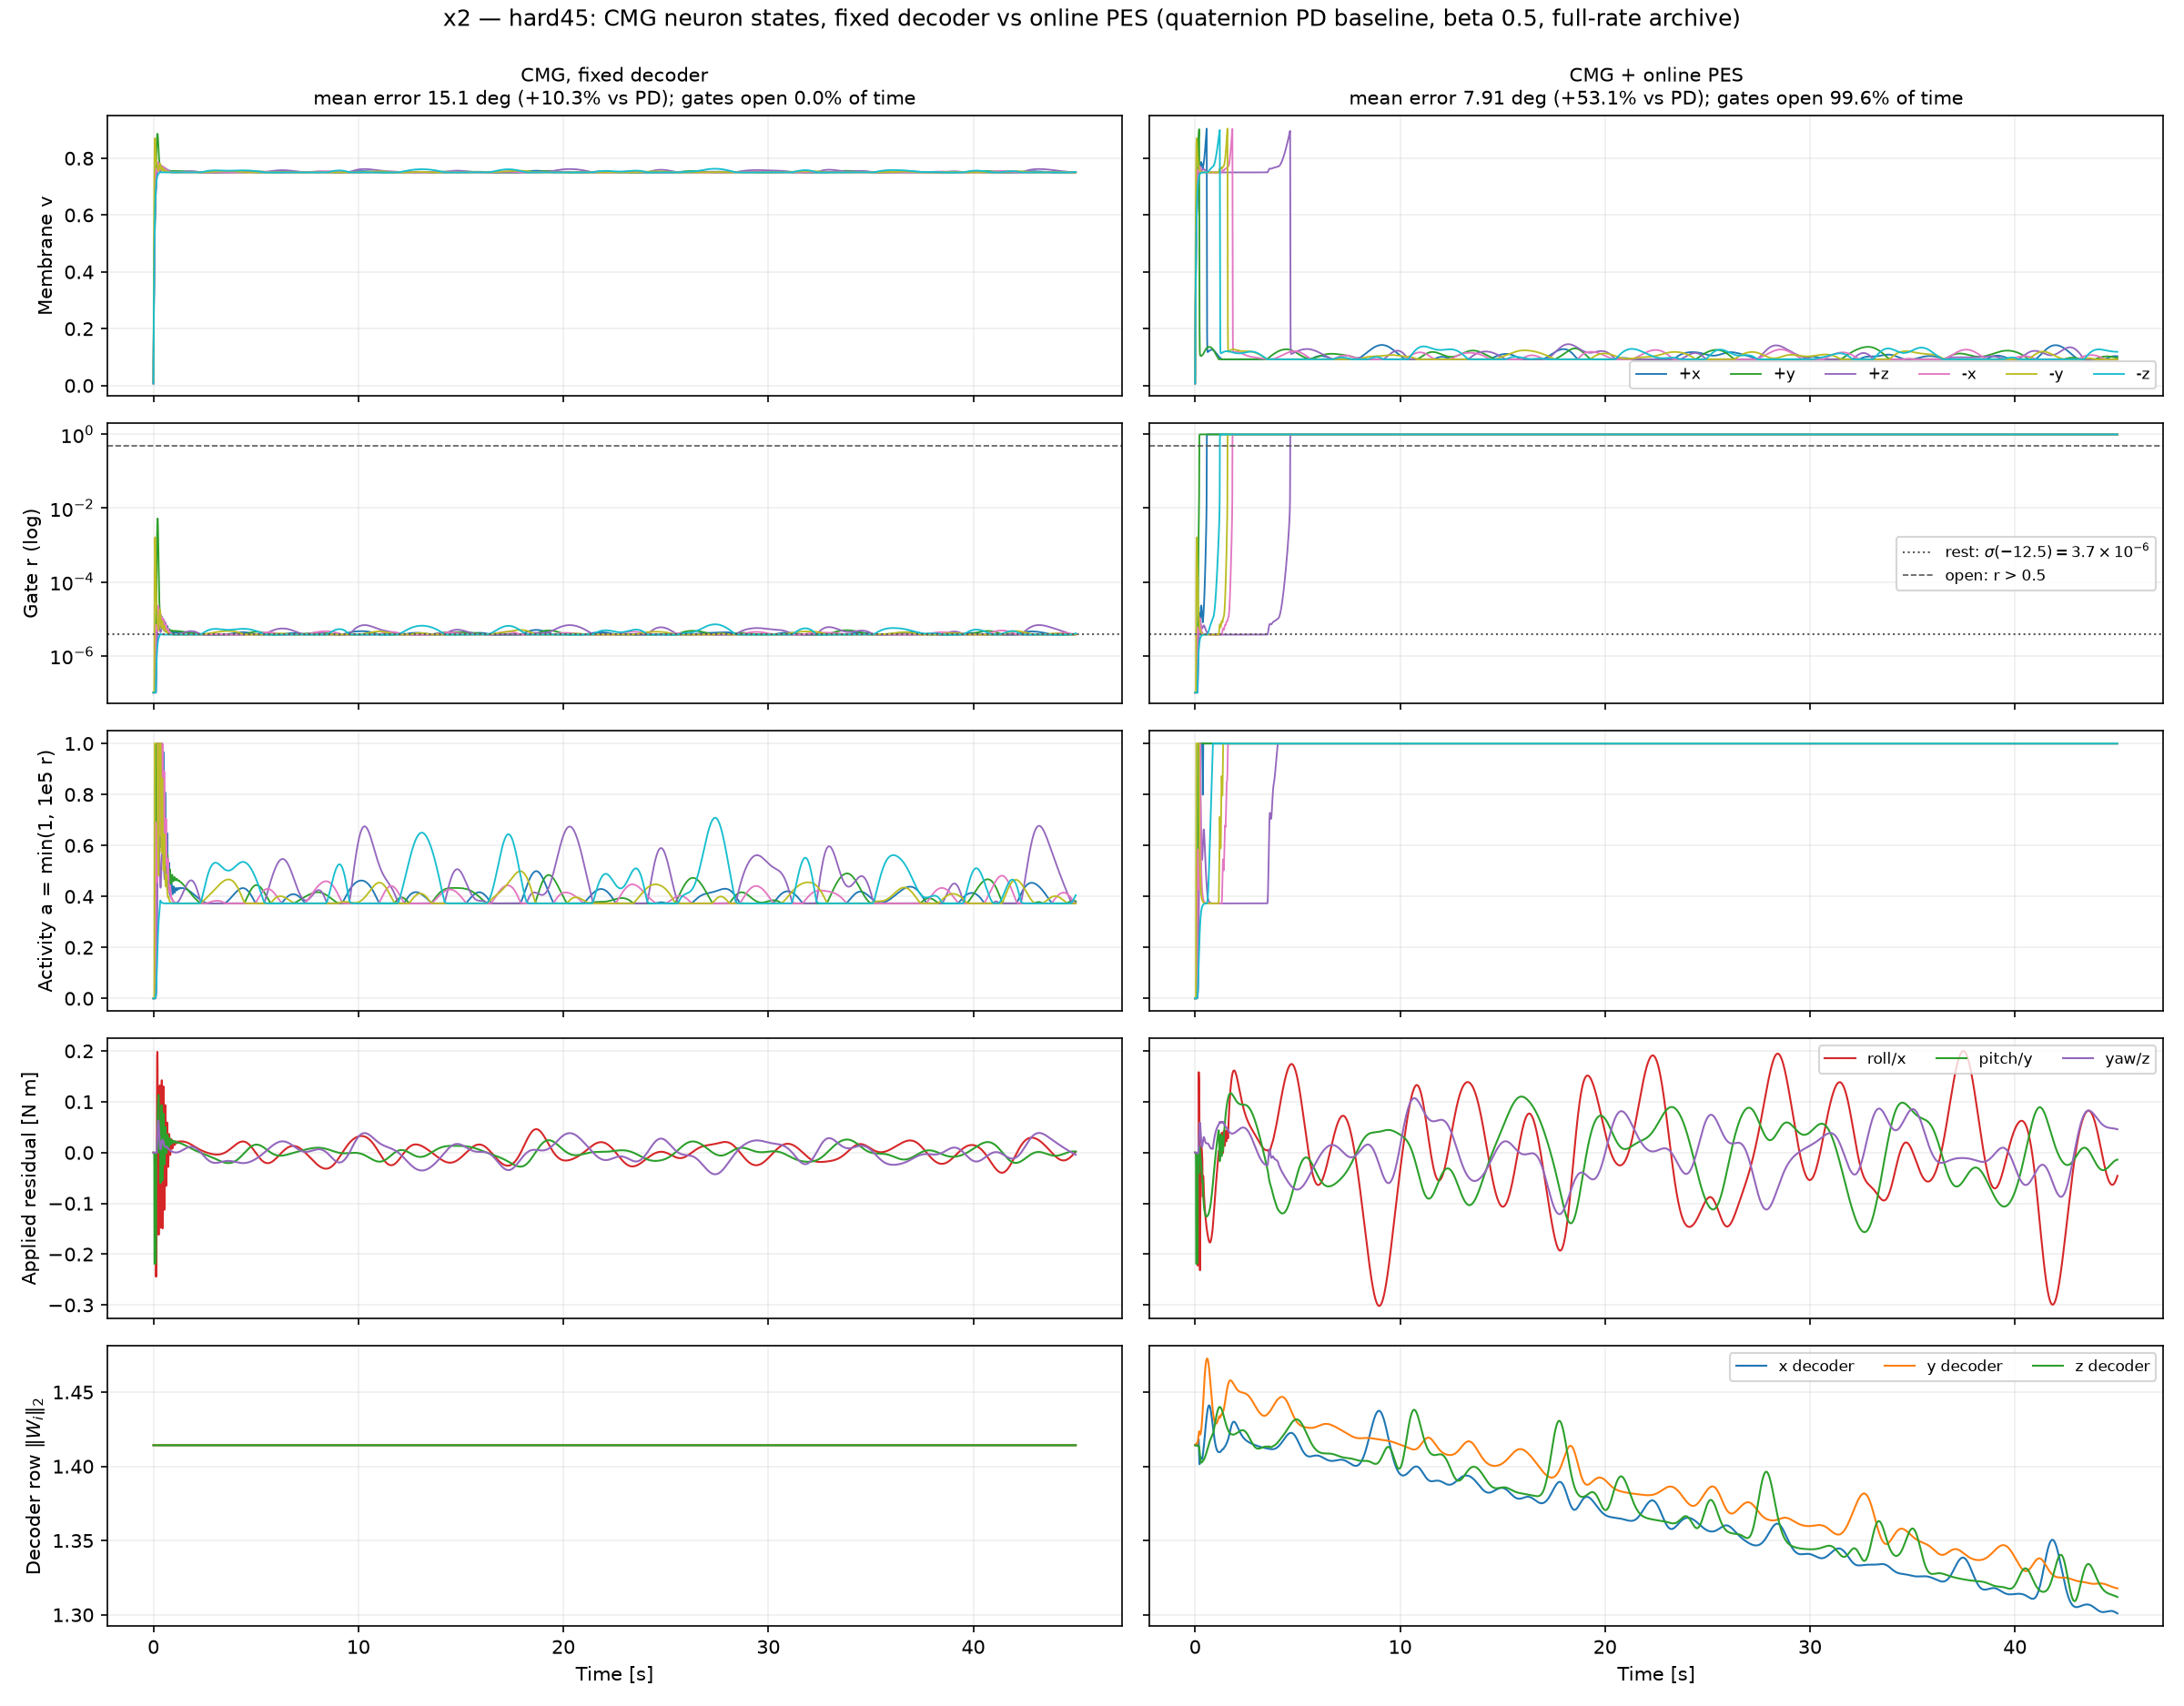
\includegraphics[width=.80\linewidth]{figures/09_CMGfixed_vs_CMGPES/x2_hard45_fixed_vs_pes.png}
\caption{X2 Hard45: internal CMG signals on the trajectory of Fig.~\ref{fig:tracking}, comparing fixed-decoder CMG (left) to online PES adaptation (right). Rows separate membrane state, raw gate $r_j$, and the clipped activity $a_j$ presented to the decoder.}
\label{fig:full3_neurons}
\end{figure*}

\subsection{Baseline Comparisons}
\label{sec:matrix}
Table~\ref{tab:all} collects every cross-mission result. Against the fixed PD
law of \eqref{eq:pd}, CMG--PES lowers mean quaternion-angle error in all ten
nominal cases, by $17.3$--$60.6\%$, while sharing the actuator interface: rotor
commands reach a bound only on Hardstep ($S=.016/.239$ on X2 and $.137/.264$ on
CF2, PD/CMG). The largest reductions occur on Yaw360 and Full3 and the smallest
on Roll. Holding the decoder at $W_k=W_0$ recovers at most a fifth of that gain,
and the reductions survive both synthetic noise levels; Yaw360 is the one cell
that loses appreciably, because its error approaches the noise floor.

The same baseline, bounded readout and allocation interface also drive four other neuron
families, in a Nengo benchmark of eleven controllers over the same ten cells: fixed and
PES variants of CMG, LIF, ALIF, Izhikevich \cite{izhikevich2003} and LIFRate, differing
only in neuron dynamics and the native-state-to-activity map. Izhikevich--PES
attains a slightly larger mean reduction than CMG--PES ($48.6$ versus $44.5\%$
geometric mean on X2), but spends three times the residual authority to do it,
and $0.25$ of the bound even with a frozen decoder. The LIF, ALIF and LIFRate
bases stay within a few tenths of a percent of the baseline outside Hardstep:
their activity is too sparse for PES to act on. Persistent temporal activity is
therefore necessary for the learning rule to have anything to shape, and the
neuron model sets the authority price of a given accuracy.

Figures~\ref{fig:tracking} and \ref{fig:full3_neurons} pair tracking
performance and internal CMG signals for X2 Hard45. Improvement refers to the
mean metric; it need not hold at every instant.

\subsection{Stronger Baselines: Feedforward and Bandwidth}
\label{sec:ladder}
The PD law of \eqref{eq:pd} damps absolute rate, so on a moving reference it
carries a velocity lag that a residual can remove without learning anything
about the plant. Repeating all ten cases on the feedforward law \eqref{eq:pdff}
separates the two effects. Feedforward alone removes $76$--$99\%$ of the
baseline error on the four moving-reference missions, and sweeping $\rho$ over
$[0.75,8]$ minimises mission-mean error at $\rho=3$ on both airframes and at
both noise levels, so the gains of \eqref{eq:pd} sit a factor of three below the
optimum of their own law. Rotor authority sets that ceiling: CF2 diverges from
$\rho=4$ upward, with a rotor at a bound in $83\%$ of samples.

The residual improves every rung of that ladder, by a shrinking margin:
$44.5/44.2\%$ over PD, $57.8/57.6\%$ over feedforward PD at $\rho=1$, and
$35.6/6.5\%$ at $\rho=3$ (X2/CF2, geometric means). Two readings deserve
emphasis. The best controller of the study is CMG--PES on the tuned baseline,
on both airframes. Yet a tuned feedforward PD by itself already beats the
PD-referenced augmented controller in every cell, by $13$--$300\times$ on the
smooth missions, so the $17.3$--$60.6\%$ headline describes \eqref{eq:pd}, not
the best classical law of this family. Realized effort falls as the baseline
improves: residual RMS on X2 Full3 drops from $.121$ to $.0216$ to
$.0148$\,N\,m across the three rungs.

Hardstep is the one mission that resists this accounting, and the reason is
kinematic rather than algorithmic. Its reference commands $63$--$111^\circ$
rotations every $2$\,s, so $97$--$99\%$ of the reported mean error is slew
transient that a bounded residual cannot remove, and the settled error is
already $3.4^\circ$ (X2) and $0.7^\circ$ (CF2). Scored by the time to enter a
$5^\circ$ band after each step, the residual delivers what the mean hides: at
$\rho=1$ it cuts settling from $1.24$ to $0.86$\,s on X2 ($-31\%$) and from
$1.18$ to $0.68$\,s on CF2 ($-42\%$). Feedforward changes nothing there, as it
must, since a piecewise-constant reference has $\bm\omega_d\equiv\bm0$.

At $\rho=3$ the sign reverses, and Hardstep is the only cell in the study where
the residual degrades performance. The mechanism follows from the latched
decoder of \eqref{eq:constantbasis}: the applied residual is a first-order
filter of its target with a $9.6$\,rad/s corner, so a loop running at
$\rho\bm\omega_n=12$\,rad/s outruns it by $72^\circ$ of phase. Meanwhile the
stiffer baseline saturates the torque box on $14$--$45\%$ of samples (X2) and
$69$--$94\%$ (CF2). On a saturated axis the interaction is one-sided: a residual
that agrees with $\bm u_0$ is clipped away and does nothing, while one that
opposes it subtracts up to $\beta\ell_i$ of authority precisely when the loop
needs all of it. The stale residual therefore brakes the slew, and settling
rises from $0.59$ to $0.83$\,s on X2.

That reading suggests its own remedy. Suppressing the residual on an axis that
is both saturated and opposed, $s_i\!\leftarrow\!0$ when $|u_{0,i}|=\ell_i$ and
$\operatorname{sgn}s_i\neq\operatorname{sgn}u_{0,i}$, leaves
$|\bm u-\bm u_0|\le\beta\bm\ell$ and exact baseline recovery untouched, and
changes nothing wherever the baseline stays inside its box. Applied to this
case it restores settling to $0.57$\,s on X2 and $0.51$\,s on CF2, below the
respective PD baselines, and keeps $\beta=0.5$ admissible on CF2, where the
ungated residual diverges. The test covers only the saturated Hardstep cells at
$\rho=3$; a systematic study under noise, disturbance and model mismatch is left
to future work, and the results reported here use the ungated law throughout.

\begin{table*}[t]
\caption{Mean $q$-error, $10^{-3}$\,rad, 45\,s; $\Delta$ = reduction over the block's own baseline [\%]; geo = geometric mean.}
\label{tab:all}\centering\scriptsize\setlength{\tabcolsep}{3pt}
\begin{tabular}{@{}lrrrrrrrrrrrr@{}}
\toprule
&\multicolumn{6}{c}{Skydio X2}&\multicolumn{6}{c}{Crazyflie~2, $1.5\times$ rotor design}\\
\cmidrule(lr){2-7}\cmidrule(l){8-13}
 & Roll & Full3 & Hard45 & Hardstep$^\dagger$ & Yaw360 & \emph{geo} & Roll & Full3 & Hard45 & Hardstep$^\dagger$ & Yaw360 & \emph{geo}\\
\midrule
\multicolumn{13}{@{}l}{\textit{PD baseline, $\bm\omega_n=(4,4,3.5)$ rad/s}}\\
PD & 50.56 & 303.28 & 294.08 & 454.53 & 75.86 & 173.12 & 51.34 & 288.38 & 285.45 & 426.18 & 75.81 & 168.68\\
\;+CMG--PES & 41.79 & 131.75 & 138.01 & 359.35 & 29.90 & 96.02 & 42.44 & 126.48 & 132.32 & 347.89 & 29.87 & 94.11\\
\;\;$\Delta$ [\%] & 17.4 & 56.6 & 53.1 & 20.9 & 60.6 & 44.5 & 17.3 & 56.1 & 53.6 & 18.4 & 60.6 & 44.2\\
\;\;$\Delta$, fixed decoder [\%] & 1.9 & 9.7 & 10.3 & 0.5 & 0.1 & 4.6 & 3.3 & 4.5 & 6.8 & 0.4 & 0.1 & 3.1\\
\;\;$\Delta$, moderate noise [\%] & 32.3 & 56.4 & 52.9 & 20.8 & 56.8 & -- & 32.4 & 55.9 & 53.4 & 18.3 & 56.8 & --\\
\;\;$\Delta$, realistic noise [\%] & 32.2 & 55.7 & 52.3 & 20.6 & 47.8 & -- & 32.5 & 55.2 & 52.7 & 18.1 & 47.8 & --\\
\midrule
\multicolumn{13}{@{}l}{\textit{Same baseline and bounded interface, other bases: $\Delta$ [\%]}}\\
\;\;Izhikevich--PES & 51.1 & 52.3 & 49.7 & 22.6 & 60.7 & 48.6 & 51.5 & 51.9 & 50.3 & 21.4 & 56.4 & 47.5\\
\;\;Izhikevich, fixed decoder & 4.6 & 4.9 & 4.6 & 0.7 & 0.2 & 3.0 & 5.6 & 5.8 & 4.0 & -2.2 & -2.2 & 2.3\\
\;\;LIF/ALIF/LIFRate, best & 0.0 & 0.0 & 0.1 & 18.5 & -0.0 & 4.0 & -0.0 & 0.1 & 0.1 & 8.4 & 0.0 & 1.8\\
\midrule
\multicolumn{13}{@{}l}{\textit{PD + rate feedforward \eqref{eq:pdff}, $\rho=1$}}\\
PD+ff & 2.98 & 72.10 & 71.02 & 454.77 & 1.78 & 26.19 & 4.91 & 42.72 & 53.18 & 425.93 & 0.74 & 20.39\\
\;+CMG--PES & 0.61 & 32.81 & 38.17 & 359.16 & 0.60 & 11.04 & 0.97 & 20.29 & 28.23 & 347.68 & 0.25 & 8.65\\
\;\;$\Delta$ [\%] & 79.5 & 54.5 & 46.3 & 21.0 & 66.4 & 57.8 & 80.2 & 52.5 & 46.9 & 18.4 & 66.4 & 57.6\\
\midrule
\multicolumn{13}{@{}l}{\textit{PD + feedforward, $\rho=3$ (bandwidth-tuned)}}\\
PD+ff & 0.34 & 10.09 & 10.54 & 265.91 & 0.20 & 4.54 & 0.56 & 7.06 & 8.65 & 262.59 & 0.084 & 3.77\\
\;+CMG--PES & 0.074 & 8.83 & 9.08 & 311.07 & 0.12 & 2.93 & 0.43 & 6.96 & 8.50 & 265.93 & 0.079 & 3.52\\
\;\;$\Delta$ [\%] & 78.4 & 12.4 & 13.8 & -17.0 & 41.8 & 35.6 & 22.9 & 1.3 & 1.8 & -1.3 & 5.6 & 6.5\\
\midrule
\multicolumn{13}{@{}p{0.985\textwidth}}{\footnotesize Realized PES residual effort, RMS as a fraction of the per-axis bound, mean over the ten cells: CMG 0.12, Izhikevich 0.37, LIF 0.04, ALIF 0.03, LIFRate 0.04; Izhikevich spends $0.25$ even with a fixed decoder, so the bases that match CMG--PES on error do so at three times its authority. Noise rows average two seeds, with seed standard deviation below $0.03$ percentage points at the realistic level. $^\dagger$Hardstep commands $63$--$111^\circ$ steps every $2$\,s, so $97$--$99\%$ of its mean error is slew that no bounded residual can remove; Sec.~\ref{sec:ladder} scores it by settling time instead.}\\
\bottomrule
\end{tabular}
\end{table*}


\begin{comment}
\begin{figure}[t]
\centering
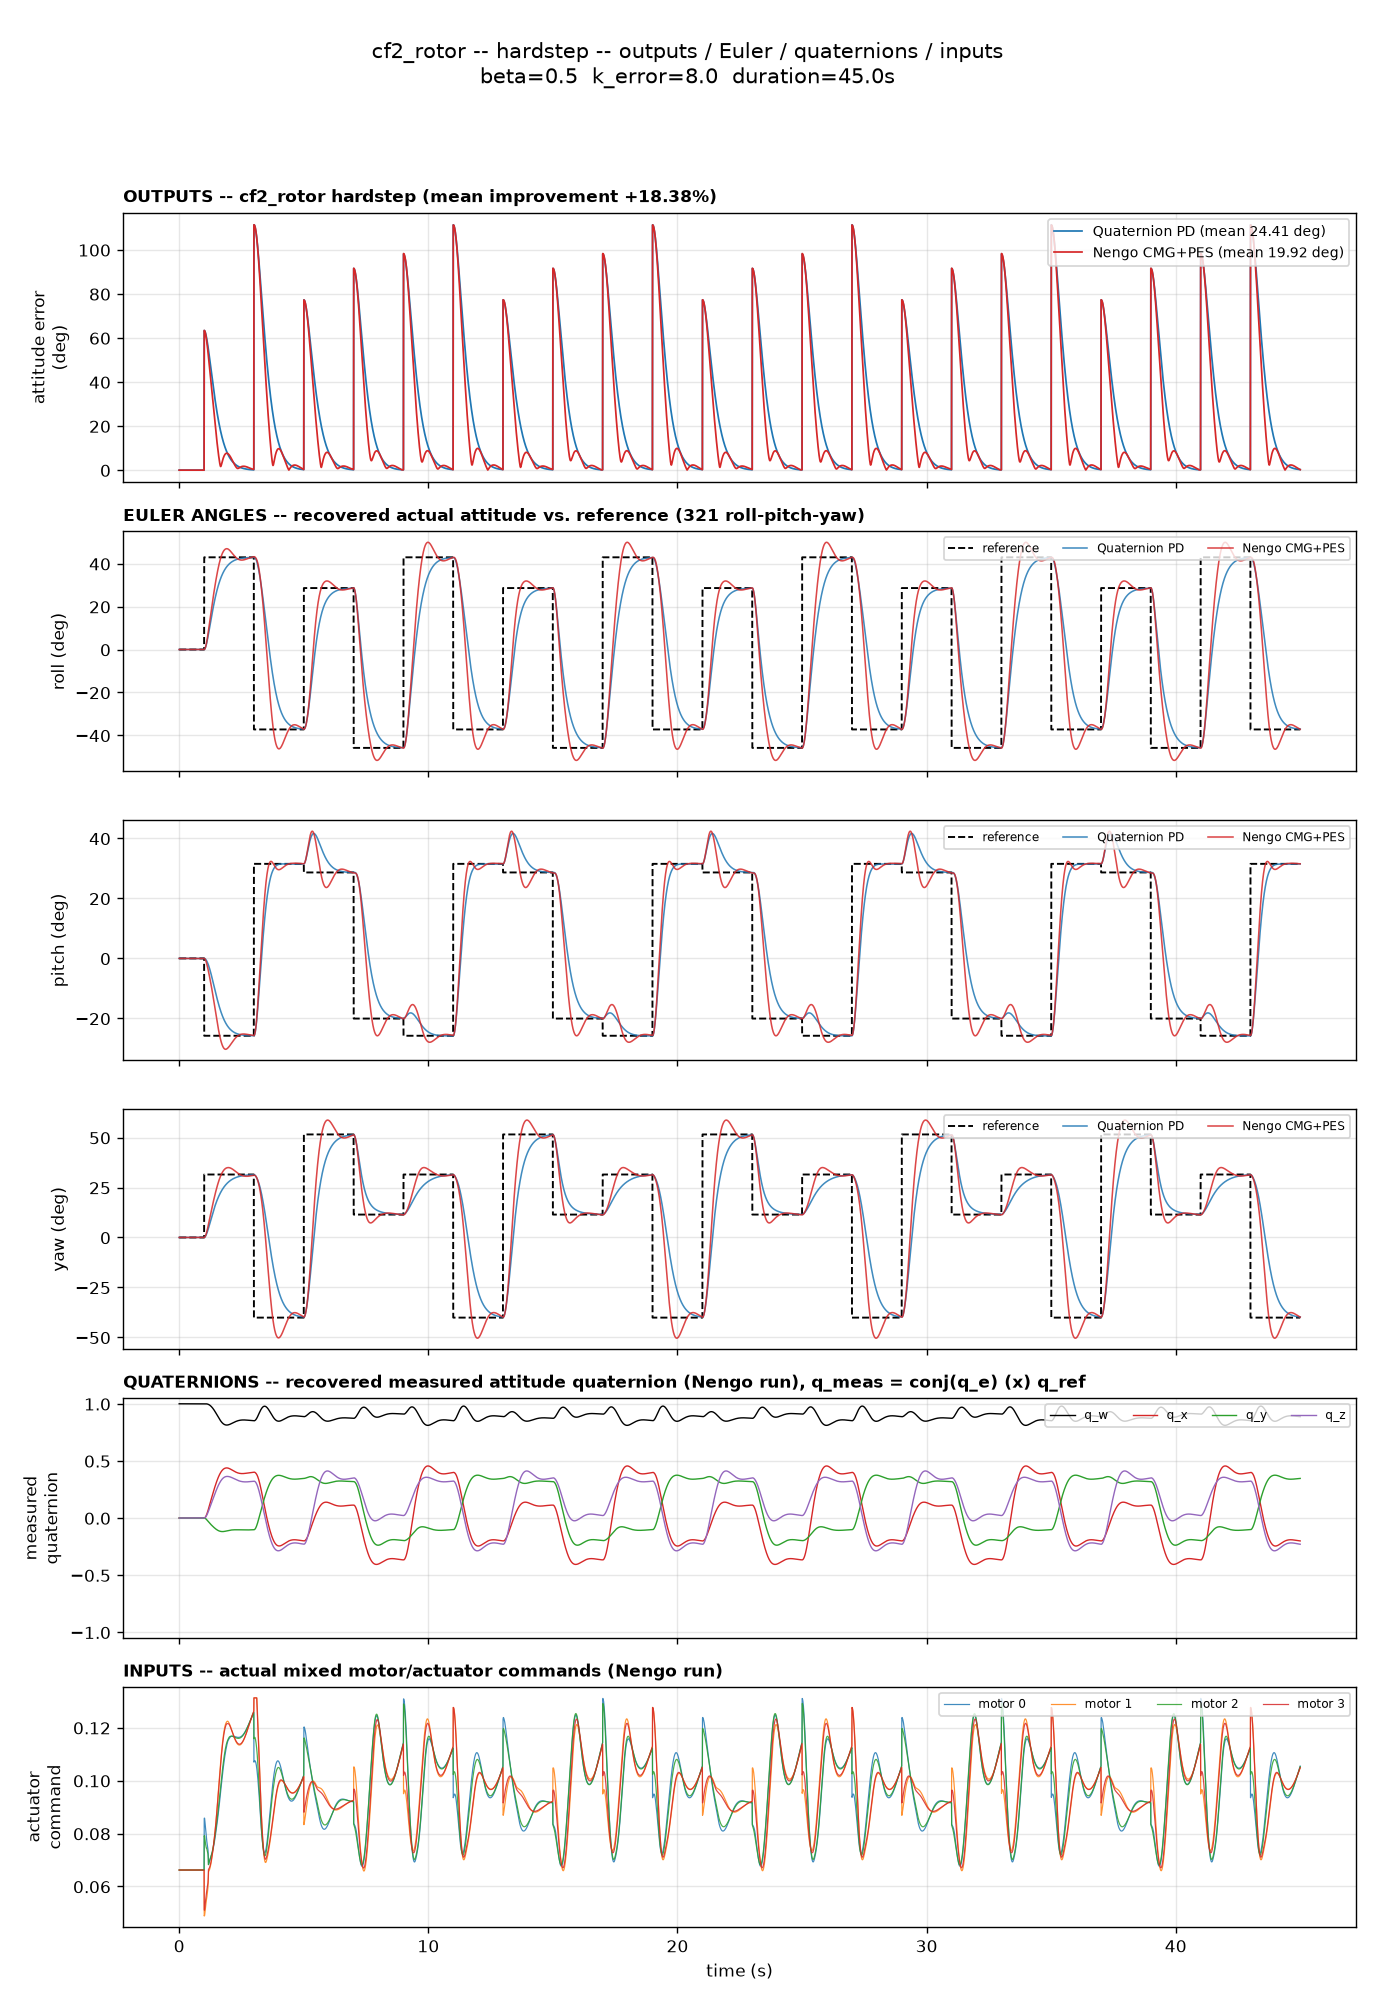
\includegraphics[width=.92\linewidth]{figures/02_neural_activity/attitude_detail/cf2_rotor_hardstep_attitude.png}
\caption{CF2 Hardstep mission: PD baseline versus CMG--PES augmentation on
the abrupt step reference. This is the hardest case in the matrix, the
smallest reduction ($18.4\%$), and the only one whose rotor commands reach a
bound ($S=.137/.264$). The residual stays inside its
authority envelope and the augmented loop remains better than the baseline
throughout.}
\label{fig:states}
\end{figure}
\end{comment}

%%%%%%%%%%%%%%%%%%%%%%%%%%%%%%%%%%%%%%%%%%%%%%%%
\subsection{Sensitivity to Measurement Noise}
\label{sec:noise}

Each of the ten cases was rerun at two synthetic noise levels with two paired
seeds: at every step independent zero-mean Gaussian samples form a small
Euler-angle quaternion left-multiplied into $q$, and additive samples corrupt
each rate component. The moderate level is $0.010$\,rad and
$0.025$\,rad\,s$^{-1}$, the realistic level $0.020$\,rad and
$0.050$\,rad\,s$^{-1}$; neither is a calibrated sensor specification. The
runner evaluates $\theta_q$ from the \emph{corrupted} quaternion the controller
uses, not from an independent ground truth, so the noise rows of
Table~\ref{tab:all} measure noisy-feedback error and inherit its floor.

All noisy reductions remain positive, spanning $18.08$--$55.75\%$ at the higher
level. Yaw360 loses about $12.8$ percentage points against clean feedback
because its error is closest to that floor, whereas Roll's relative reduction
increases. Seed standard deviations are $.001$--$.101$ pp at the moderate level
and $.002$--$.031$ pp at the realistic one: limited repeatability, not a
population confidence interval.

\begin{comment}
\begin{figure}[t]
\centering
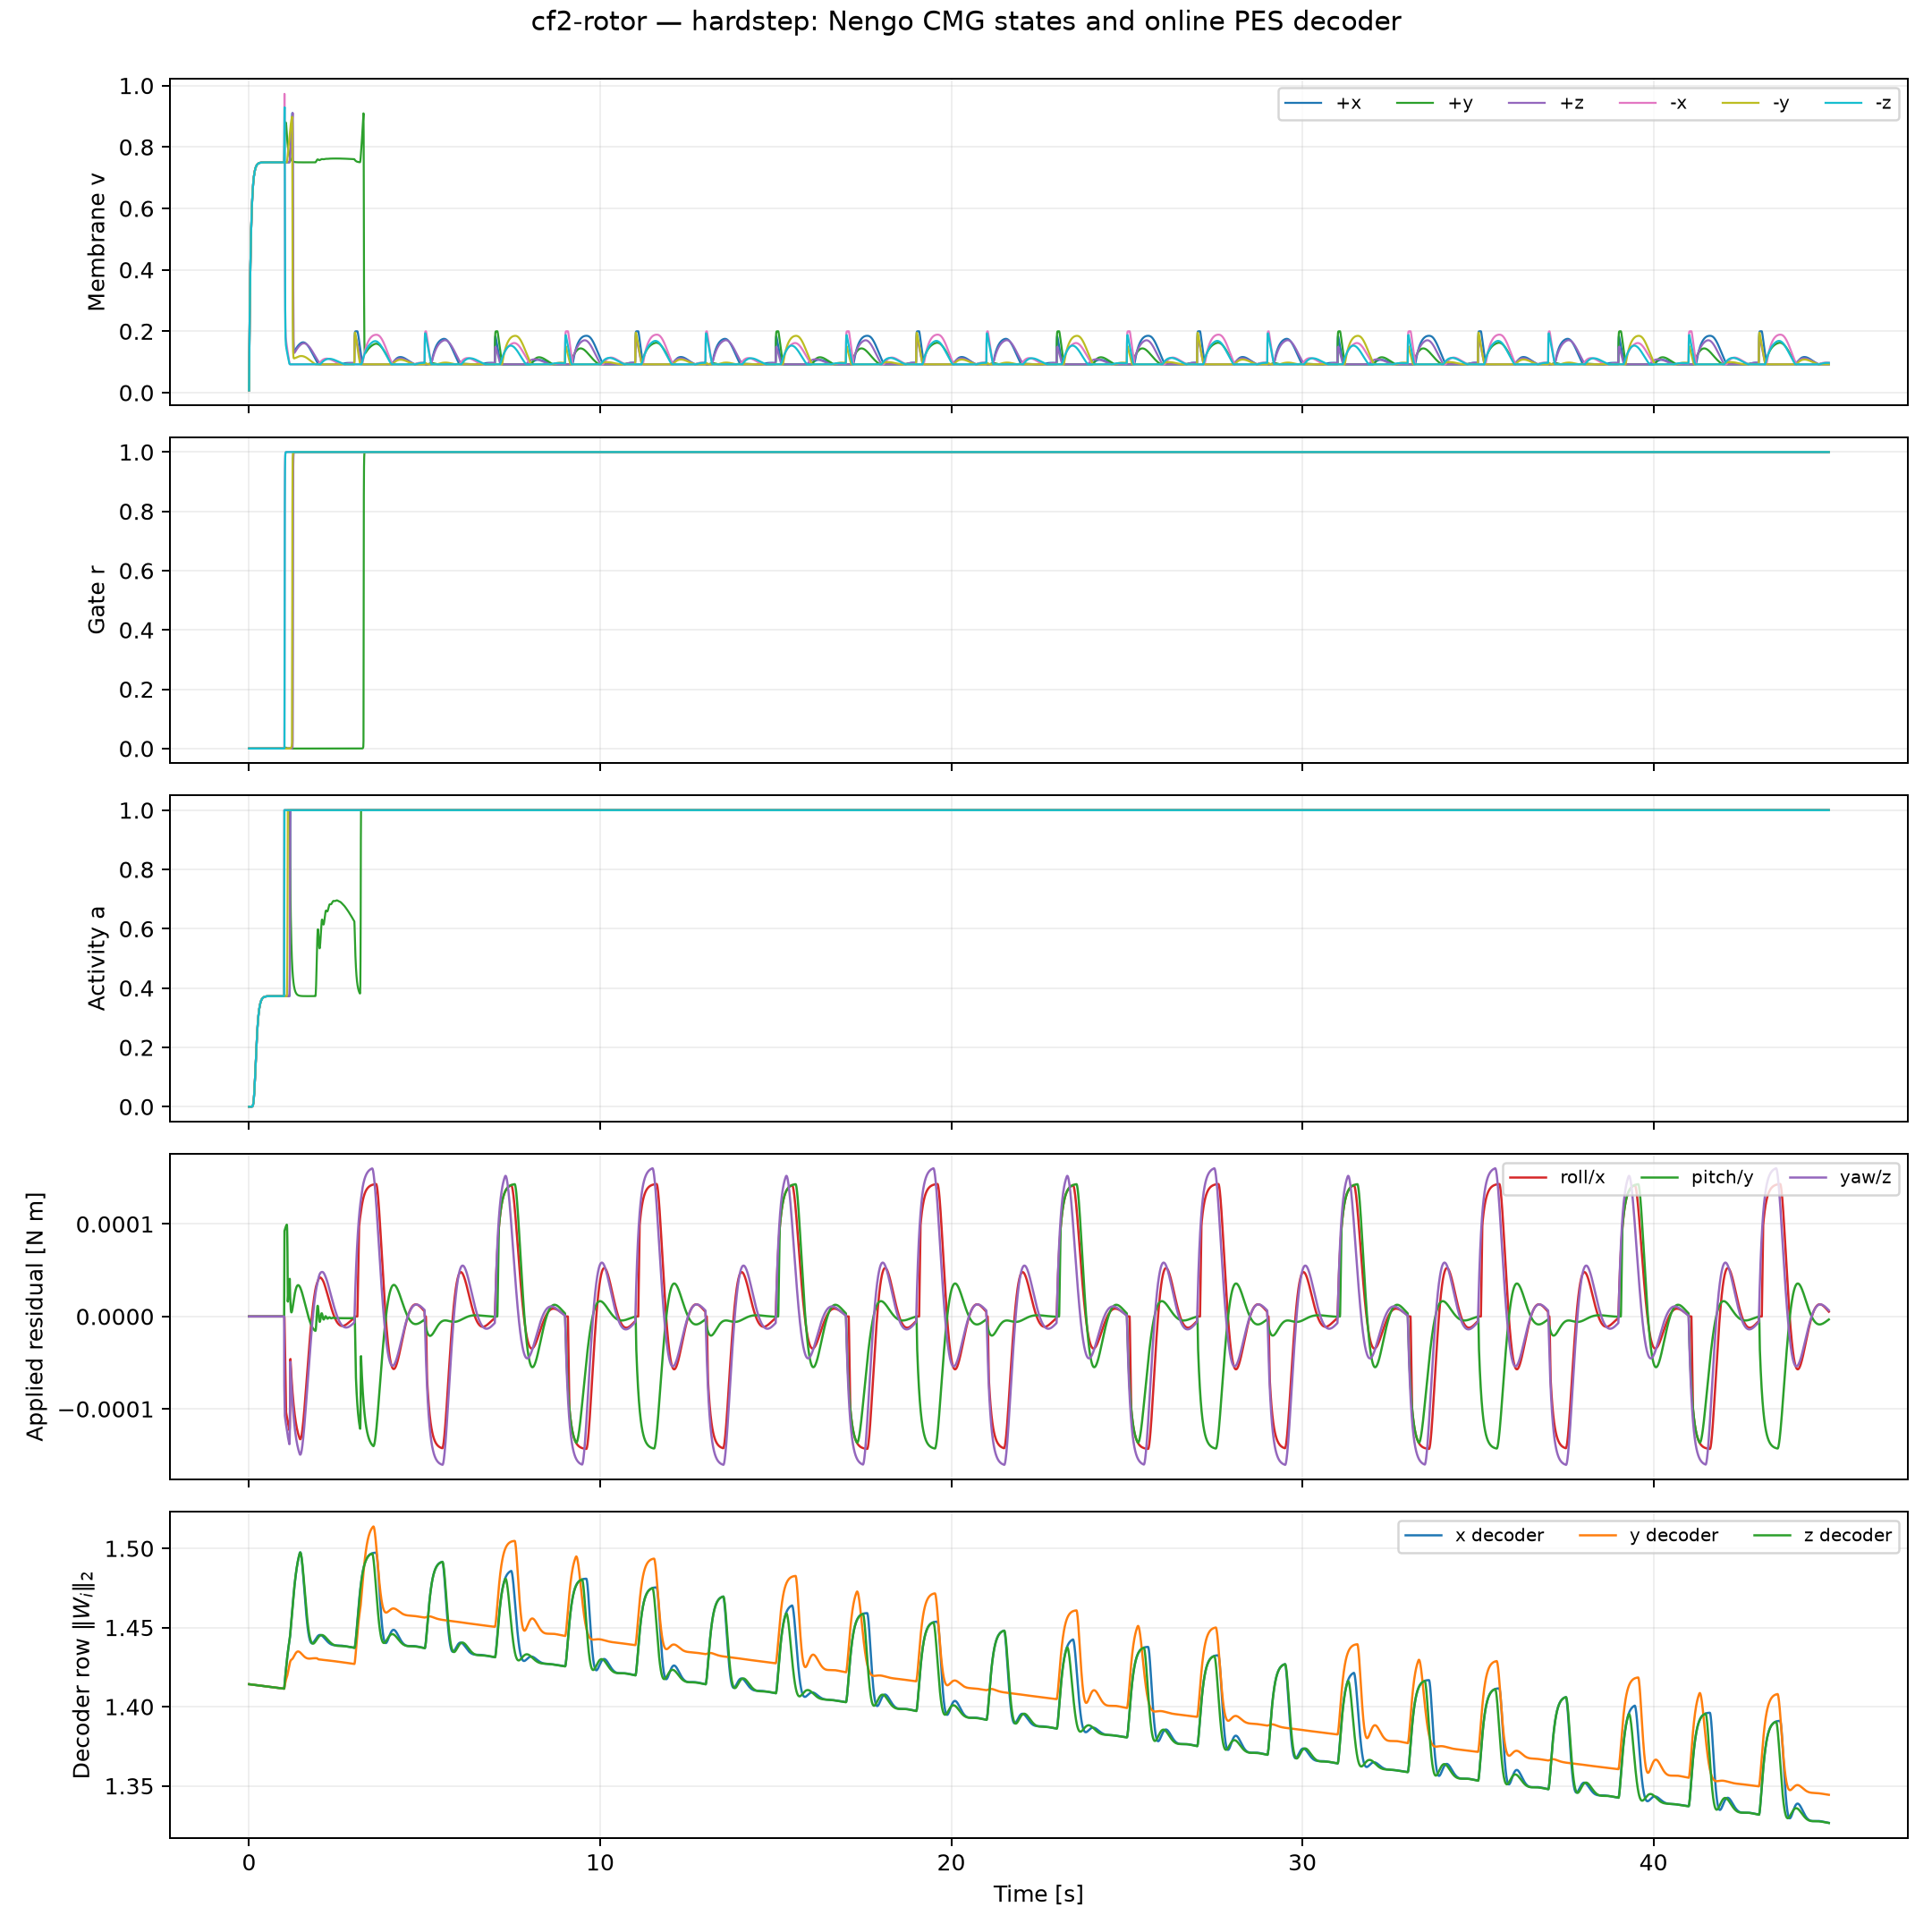
\includegraphics[width=\linewidth]{figures/02_neural_activity/cf2-rotor_hardstep_neurons.png}
\caption{CF2 Hardstep: internal CMG signals on the same trajectory as
Fig.~\ref{fig:states}. The plot separates membrane state, raw gate $r_j$, and
the clipped activity $a_j=\clip_{[0,1]}(Gr_j)$ presented to the decoder,
illustrating the readout saturation of Sec.~IV-D under the one mission that
also drives the rotors to a bound.}
\label{fig:cf2_hardstep_neurons}
\end{figure}
\end{comment}

%%%%%%%%%%%%%%%%%%%%%%%%%%%%%%%%%%%%%%%
\subsection{Ablation: What Drives the Improvement?}\label{sec:ablation}

We separate decoder adaptation (PES), input-dependent conductance
modulation ($\chi$), and readout gain ($G$). Toggling $\chi$, which
retains the base shunt $g_0r_j^2$, is numerically indistinguishable with
the decoder mode held fixed. \emph{Fixed versus adaptive decoder.} Holding $W_k=W_0$ keeps the neuron
dynamics but reduces the readout to $\bm a^+-\bm a^-$, a bounded, stateful
image of the PD request. It still helps (X2 $0.12$--$10.27\%$, CF2
$0.06$--$6.80\%$; Table~\ref{tab:all}), so fixing the decoder does not
remove \emph{all} improvement, yet it recovers at most a fifth of the PES
gain in any cell. Fig.~\ref{fig:full3_neurons} shows why, row by row.
\emph{Membrane and gate.} At $I_j=I_b$ the membrane rests at
$v_j\approx0.75<v_{\rm th}$, so
$r_j=\sigma(\alpha_h(I_b-v_{\rm th}))=\sigma(-12.5)\approx3.7\times10^{-6}$:
the gate is deep in its logistic tail, not closed. Once $r_j\ge1/2$,
$\gamma=2$ and $v_j\ge0$ (Proposition~\ref{prop:states}) give
$b_{j,k}\ge1/2$ in \eqref{eq:gate_step}, so an opened gate cannot close
(none did in the twenty runs), and the shunt holds $v_j$ near $0.09$.
\emph{Activity.} With $G=10^5$ the resting gate already gives
$a_j\approx0.37$, graded by the input; a latched gate pins $a_j=1$. With
the fixed decoder only the $\pm y$ pair latches on Full3 (both models), so
$a^+_y-a^-_y=0$ and the pitch residual is exactly zero after 1\,s while
the sub-threshold units carry roll and yaw. Under PES on X2,
$\bm a_k\equiv\bm1$ from $2.02$\,s (all gates latched by $2.4$\,s), and
for constant $\bar{\bm a}$ with inactive projection the direct update
gives $\bm z_k=W_k\bar{\bm a}$ the recursion
\begin{equation}
 \bm z_{k+1}=(1-\lambda_W)\bm z_k
 +\eta\|\bar{\bm a}\|^2[\bm y_k^*-\clip_{[-1,1]}(\bm z_k)],
 \label{eq:constantbasis}
\end{equation}
the leaky constant-feature regime of Proposition~\ref{prop:pes}: a
first-order filter of the teaching target with pole $0.9952$, a time constant
of about $0.10$\,s and hence a corner near $9.6$\,rad/s, while the readout clip
is inactive. That corner is what separates the bandwidths in
Sec.~\ref{sec:ladder}.
\emph{Residual and decoder.} The residual RMS rises from $0.026$ to
$0.123$\,N\,m and the decoder moves $\|W_T-W_0\|_F=0.37$; on Roll, Full3,
Hard45, and Hardstep PES applies $4$--$12\times$ the fixed residual RMS on
both models. Where no gate opens (Roll, Yaw360; $r_j\le1.6\times10^{-3}$)
PES lifts the driven membranes toward threshold ($v_j\le0.87$) and uses
the graded tail. Decoder adaptation is therefore the principal lever: the
CMG dynamics supply a bounded basis, latched or graded, on which PES
shapes the correction.

%We distinguish decoder adaptation (PES), input-dependent conductance modulation ($\chi$), and readout gain ($G$). Toggling $\chi$ retains the base shunting term $g_0r_j^2$; it is not removal of all conductance or all CMG dynamics.
%Fixed-decoder residuals already improve some missions: in the audited direct
%X2 runs their mean reductions range from about 0.12\% to 10.27\%; the
%corresponding CF2-design range is 0.06\% to 6.80\%. Thus it is inaccurate
%to say that fixing the decoder removes \emph{all} improvement. PES produces
%the much larger 17.3--60.6\% primary reductions. Separately, toggling
%$\chi$ with the decoder mode held fixed is numerically indistinguishable
%under the tested settings. Decoder adaptation is therefore the principal lever in the tested regime.

%Readout saturation does not imply negligible conductance. In the fresh canonical X2 Full3 rerun, $r_j>0.9$ for $97.7\%$ of unit-samples and mean $c_j\tau$ is $7.08$. Yet $a_j$ clips at $r_j=10^{-5}$.
%Moreover, with $\gamma=2$ and $v_j\ge0$, $r_j\ge1/2$ implies $b_j\ge1/2$ in \eqref{eq:gate_step}; its convex update preserves that high-gate region. Conductance can therefore change membrane voltage without producing a distinguishable decoded activity.

%The resulting decoder has a useful exact reduction. On an interval with
%$\bm a_k=\bar{\bm a}$ and inactive weight projection, let
%$\bm z_k=W_k\bar{\bm a}$. Then \eqref{eq:pes} gives
%\begin{equation}
% \bm z_{k+1}=(1-\lambda_W)\bm z_k+
% \eta\|\bar{\bm a}\|^2[\bm y_k^*-\clip_{[-1,1]}(\bm z_k)].
% \label{eq:constantbasis}
%\end{equation}
%When readout clipping is inactive, this is a first-order target filter.
%For six unit activities its pole is $.995199$, corresponding to about
%$.104$ s. This is a direct-backend identity under the stated conditions,
%not equivalence of the full transient CMG or delayed Nengo dynamics.
%The recorded X2 Full3 activity is identically one after $2.02$ s; the
%reduced recursion matches its saved decoder to $8\times10^{-16}$.

%A focused direct-backend sweep uses $G\in\{1,10^3,10^5,10^6\}$ and $\chi\in\{0,1\}$ on X2 Full3 and CF2 Hardstep. Their reductions remain $56.04$--$56.97\%$ and $18.34$--$18.46\%$, respectively. In contrast, X2 Roll ranges from effectively zero at $G=1$ to $17.36\%$ at $10^5$ and $57.76\%$ at $10^6$ (also tested at $10^2,10^4$). These are fixed-$\eta$ sensitivity tests: before clipping, same-feature PES excitation scales as $\eta G^2\|\bm r\|^2$. They do not isolate neuron expressiveness. Eight selected Nengo checks agree with the direct mean errors to relative difference $1.13\times10^{-7}$.

%\begin{table}[ht]
%\centering\footnotesize
%\caption{Direct-backend controls: mean-error reduction over matched
%PD [\%]. Same $W_0$, PES teacher/update, leak, caps, and allocation;
%canonical CMG uses $G=10^5$. One deterministic run per cell.}
%\label{tab:simplebasis}
%\setlength{\tabcolsep}{4pt}
%\begin{tabular}{lrrr}
%\toprule
%Case & CMG & Paired-linear & Constant\\\midrule
%X2 Roll &17.36&0.73&57.78\\
%X2 Full3 &56.56&6.70&56.98\\
%CF2 Hardstep &18.37&1.50&18.38\\\bottomrule
%\end{tabular}
%\end{table}

\begin{figure}[ht]
\centering
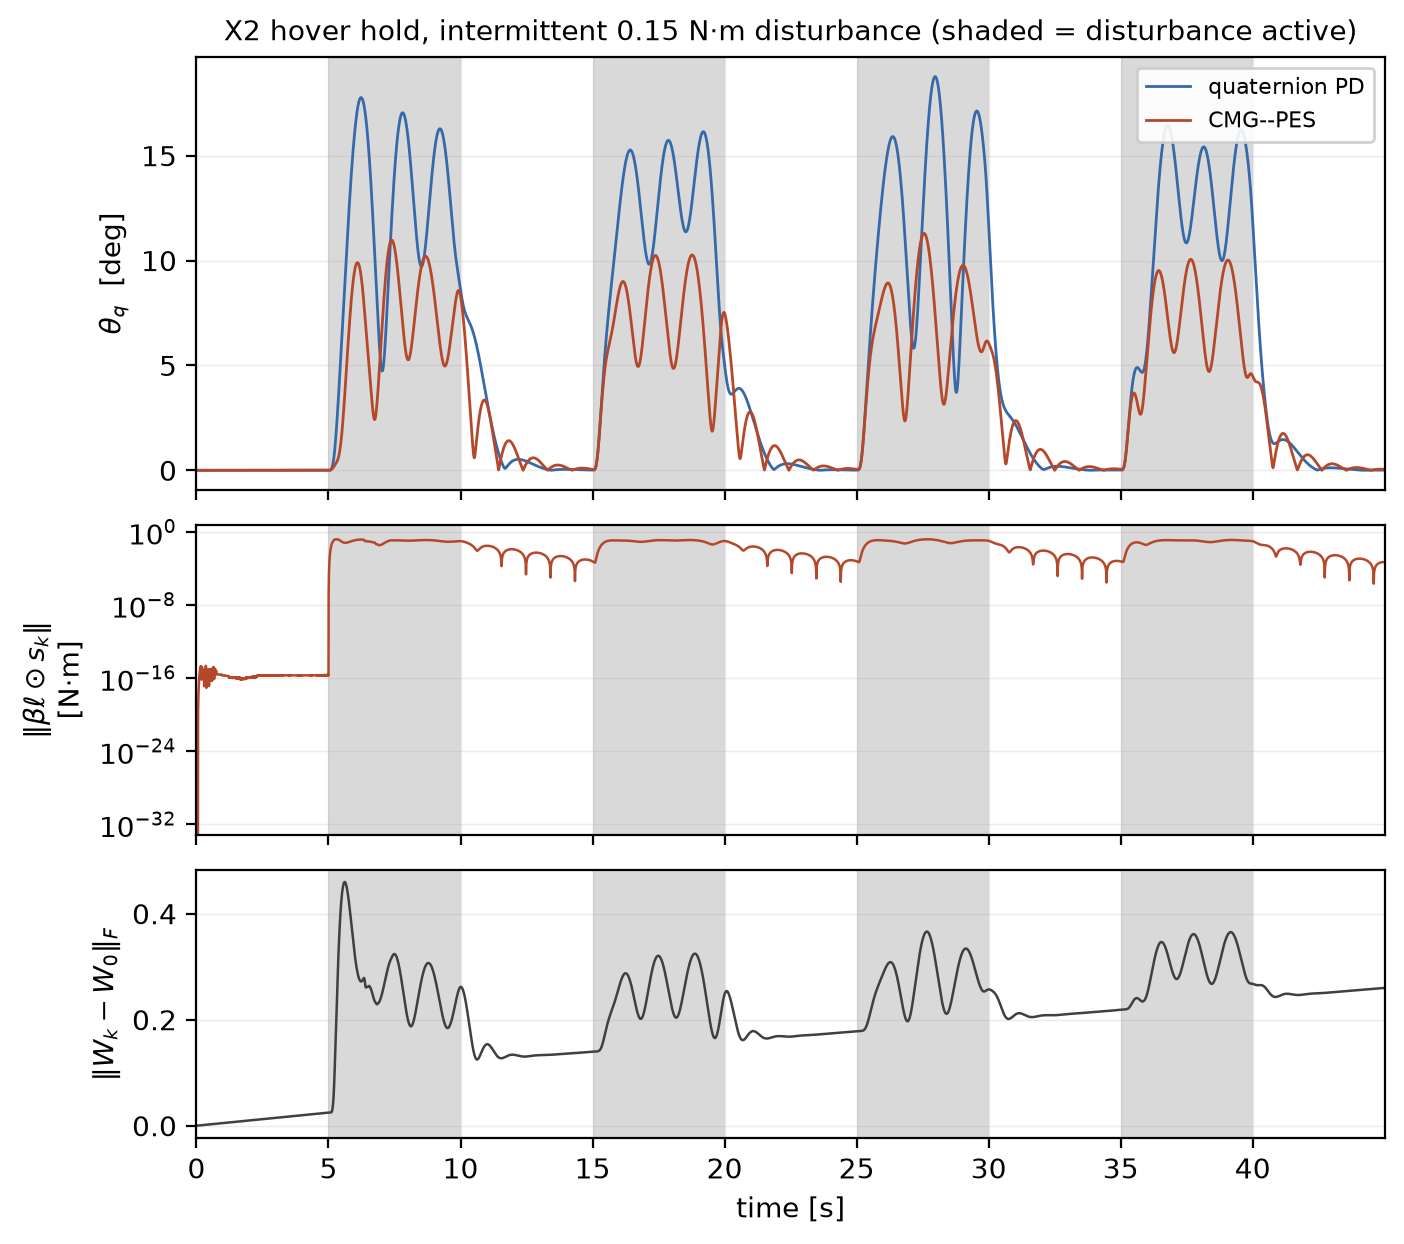
\includegraphics[width=.88\linewidth]{figures/07_disturbance_and_noise/hover_intermittent.png}
\caption{X2 hover hold under four $0.15$\,N\,m disturbance bursts (shaded)
separated by quiet intervals. Top: attitude error. Centre: residual
magnitude, logarithmic. Bottom: decoder displacement from $W_0$. The
residual is at numerical precision before the first burst. This means
negligible initial correction, not zero computation or energy cost.}
\label{fig:hover_int}
\end{figure}

%%%%%%%%%%%%%%%%%%%%%%%%%%%%%%%%%%%\subsection{Disturbance Rejection and Retention}
\label{sec:disturbance}
An equilibrium test applies
$\bm\tau_{\rm d}=d_b\rho(t)[\sin(1.31t+.2),\allowbreak
.8\sin(1.73t+1.1),\allowbreak.6\sin(2.17t+2)]\T$ in body axes.
After 5 s of quiet, $\rho$ alternates 5-s on/off intervals with 0.25-s
raised-cosine edge ramps. For X2, $d_b=.15$ N\,m is the first component's
amplitude, not a vector-norm bound.
The four-burst 45-s experiment (Fig.~\ref{fig:hover_int}) cuts burst-phase
mean error from $11.50^\circ$ to $6.65^\circ$ ($42.2\%$) and post-burst
quiet error from $1.21^\circ$ to $.99^\circ$ ($18.0\%$).
The CF2 rerun uses $d_b=.00015$ N\,m (a selected scaling, not an exact
inertia-ratio match); its full-run mean falls from
$.141199$ to $.070259$ rad ($50.24\%$).

%The 180-s X2 record contains eighteen bursts and seventeen complete post-burst quiet intervals, not sixteen bursts. Decoder displacement reaches $.797$ at the final sample, with maximum absolute weight $1.089$.
%One quiet interval is about $4\%$ worse than PD. Continued weight change and nonzero quiet-phase errors do not establish convergence. Because learning and leakage remain active, and the multi-sine phase is not reset between bursts, this study shows persistent adaptation, not causal proof of reuse without relearning. A reset-decoder or frozen-decoder control is needed to test that hypothesis.

\section{Discussion and Conclusion}
\label{sec:conclusion}
% [v7] Rewritten: states the positive result once and plainly, keeps the
% limits in one place instead of after every sentence, and separates the
% analog outlook from the claims.

A bounded residual of six continuous CMG units and eighteen PES-adapted decoder weights augments a fixed quaternion PD baseline without changing its gains or actuator interface, reducing mean quaternion-angle error by $17.3$--$60.6\%$ over ten matched 45-s MuJoCo cases on two modeled platforms, within rotor saturation and with exact baseline recovery at zero authority; direct and Nengo realizations agree to $2.013\times10^{-6}$ relative mean error.

Decoder adaptation is the dominant source of improvement in the tested regime: a fixed decoder gives at most $10.3\%$, and toggling $\chi$ is indistinguishable. Opened gates latch and saturate the readout, where a fixed paired decoder can cancel an axis, while sub-threshold units stay in a graded logistic tail; PES shapes the correction on either basis. Across all five neuron families PES is the consistent differentiator, and the dynamics mainly set an effort--accuracy tradeoff. The readout gain $G$, which sets the resting activity at $0.37$, is a key sensitivity parameter.

Limitations: results are in simulation (Sec.~\ref{sec:noise} bounds noise sensitivity; model mismatch and hardware effects are not addressed), the retention horizon is limited, and bounded commands, states, and weights are implementation properties, not global stability proofs.

Future work includes integral-action and matched-stiffness baselines, a systematic study of the saturation-gated residual of Sec.~\ref{sec:ladder} under noise, disturbance and model mismatch, matched-effort comparisons against non-neural bounded bases, sweeps of $G$ and $\chi$, longer retention studies, held-out evaluations with frozen learned weights, full 6-DOF extension, and, most importantly, validation on physical aerial, ground, and other robotic platforms; the same bounded-residual wrapper extends to nonlinear and optimal-control baselines with hard actuator constraints.


%A bounded neuromorphic residual can augment a fixed quaternion PD baseline without changing its gains or actuator interface. Using six continuous CMG units with eighteen PES-adapted decoder weights, the augmented loop reduces mean quaternion-angle tracking error by $17.3$--$60.6\%$ over ten matched 45-s MuJoCo cases on two modeled platforms, while respecting rotor saturation and recovering the baseline exactly at zero residual authority. Direct and Nengo realizations agree to $2.013\times10^{-6}$ relative mean error.

%Mechanism studies show that, in the tested regime, decoder adaptation is the dominant source of improvement: fixed-decoder residuals yield only modest reductions, and toggling the input-dependent conductance term ($\chi$) with the decoder mode held fixed is numerically indistinguishable. Across CMG, LIF/ALIF, Izhikevich, and LIFRate bases, PES is the consistent differentiator, while neuron dynamics mainly set an effort--accuracy tradeoff (matching error often requires substantially more residual effort). The observed readout saturation $a_j=\clip(Gr_j,0,1)$ suggests $G$ is a key sensitivity parameter.

%Limitations: results are in simulation (Sec.~\ref{sec:noise} bounds noise sensitivity, but model mismatch and hardware effects are not addressed); the repeated-disturbance retention horizon is limited; and bounded commands, states, and weights are implementation properties rather than closed-loop stability proofs.

%Future work will include integral-action baselines, matched-effort comparisons against non-neural bounded bases, systematic sweeps of $G$ and $\chi$, longer-horizon retention studies, held-out evaluations with frozen learned weights, extension to full 6-DOF systems, and, most importantly, validation on physical robotic platforms, including aerial, ground, and other dynamical systems. The same bounded-residual wrapper can also be extended to nonlinear and optimal-control baselines subject to hard actuator constraints.



% Finalize human authors, affiliations, funding, and any required tool-use
% disclosure before submission. No invented author identities are supplied.
\bibliographystyle{IEEEtran}
\bibliography{references}
\end{document}
